\chapter{TRACKING PROTOCOLS}
\label{Section: Tracking Protocols}

We consider two scenarios to study tracking protocols in tag-based information systems. We call the first one \emph{space-time correlations}, and this applies to a variety of situations. The second scenario is a specific search and rescue system in a forest setting. In the first scenario, we inherently assume that tags have infinite storage space, while in the second, we assume tags have finite storage space.

\section{Space-Time Correlations}
\label{Section: Tracking Protocols: Space-time Correlations}
Consider passive tags distributed densely in space. Users equipped with interrogators move through the tag field, continuously scanning the tags.  As a user moves, stationary tags enter and exit her scan range (relative to her position).  A subset of tags are said to be \emph{space-time correlated} with respect to the user's trajectory.  The correlation value is high if the tags are close together in space and are scanned by the user close together in time.  The correlation also has a direction, indicating the movement of the user in that space-time locality.  This correlation value and direction form a virtual arrow. Consider two tags being scanned. The value (arrow weight) is stored in either or both of the two tags, and the direction is stored by writing the second tag's ID into the first tag (and possibly vice versa).  These weighted arrows form a digital path of the user for localization and tracking. This general scenario is applicable in many different situations. For example, tags can be embedded beneath the floor tiles or inside the walls of a large office building. As people equipped with interrogators move through the building, they can leave digital paths, as well as follow paths of other people. In another example, robots in a warehouse or factory can both leave digital paths and follow them. Therefore, we see that the sizes of the potential pervasive spaces for this situation are similar to Super Spaces in \cite{2004 Al-Muhtadi}.

In this section, we consider several methods of forming these digital paths. We perform experiments to actually create them. We study the paths from a tracking perspective as well as a search and rescue perspective.

\subsection{System Model}
Consider a large set of passive tags, $\mathcal{T}$, distributed in space.  Each tag has position $\mathbf{p}_i$, where $i \in \mathcal{T}$.  We assume each tag has a large storage memory (relative to the application requirements).  (The TegoChip has 32 kilobytes \cite{Tego}.)  That is, our system is not storage-limited.\footnote{In Section \ref{Section: Tracking Protocols: Forest Search and Rescue}, we consider a system where tags are storage-limited.  Users thus may choose to replace existing information in a tag.  We investigate \emph{replacement algorithms} in this later section.}  Each tag is identified by a unique ID $u_i$, which is stored in the tag itself.  The position $\mathbf{p}_i$ may also be stored in the tag.  Users, each equipped with an RFID interrogator, move through the tag field and scan the tags, reading from and writing to them.  The set of users is $\mathcal{R}$. 

\subsection{Correlation Functions}
\label{Section: Tracking Protocols: Space-time Correlations: Correlation Functions}
Users exploit the space-time correlations of scanned tags as they move through the tag field according to various trajectories.  For example, if a user with a small scan range scans two tags within a short time period, they are highly correlated to each other in both space and time (with respect to that user at that point in her trajectory).  We can then store a virtual arrow with a large weight in the two tags, pointing from the earlier scanned tag to the later scanned tag.  At a later time, if another user encounters this arrow, she can confidently guess that the previous user moved in the arrow's direction at this position in the past.

The positions of tags may be stored in the tags themselves.  Or, users may have a map $M:u_i \rightarrow \mathbf{p}_i$.  In either case, users can determine a tag's position by scanning its ID.  If the positions are unavailable, a user may estimate relative tag positions $\hat{\mathbf{p}_i}$ (distance between tags), for example, using her scan range.  Alternatively, tag positions may not be used at all.  Assuming users are continuously scanning tags, let $t^{\left(in\right)}_{i,r}$ and $t^{\left(out\right)}_{i,r}$ be the times when tag $i$ enters and exits the scan range of user $r$ during her trajectory, respectively, where $r \in \mathcal{R}$.  Note that tags are assumed stationary, and users are mobile. So entering and exiting are with respect to the user's frame of reference. Envisioning tags moving into and out of users' scan ranges provides greater insight to the situation.  (For simplicity, we assume a user encounters a tag only once in her trajectory.  Otherwise, we would require enter and exit times for each encounter.)  In general, user $r$ progressively acquires these space and time values (i.e. $\mathbf{p}_i$, $t^{\left(in\right)}_{i,r}$ and $t^{\left(out\right)}_{i,r}$) as she moves, which can be mapped through a correlation function $\mathbf{f}$, into weighted directions (arrows).  These arrows are stored in the tags, to be queried later possibly by other users.  This general setup allows for a large class of correlation functions.  That is, a user can use her entire history of tag scans to calculate many different correlations.  However, for practical implementation's sake, we consider six correlation functions, where at time $t$, user $r$ only uses the set of tags  being currently scanned, $\mathcal{T}\left( t \right)$.  (That is, these are the tags within her current scan range.)  There are three possible weightings and two possible directions for the correlation functions.  The weightings are
\begin{eqnarray}
w^{\left(equ\right)}  = 1,
\label{Equation: Correlation Weight1}
\end{eqnarray}
\begin{eqnarray}
w^{\left(num\right)}  = \left| \mathcal{T} \left( t \right) \right|,
\label{Equation: Correlation Weight2}
\end{eqnarray}
and
\begin{eqnarray}
w^{\left(inv\right)} = \frac{1}{ \max_{i,j} \left( t^{\left( in \right)}_{i,r} -  t^{\left( in \right)}_{j,r}\right)}.
\label{Equation: Correlation Weight3}
 \end{eqnarray}
Weighting $w^{\left(equ\right)}$ gives equal weight to all arrows, $w^{\left(num\right)}$ gives more weight to arrows when more tags are being scanned, and $w^{\left(inv\right)}$ gives more weight to arrows when the tags being scanned are closer in time.  (That is, the weight is inversely proportional to the maximum entrance time difference of tags currently being scanned.)  Intuitively, these latter two weightings put more emphasis on arrows when tags are relatively denser in space and time.  The directions are
\begin{eqnarray}
\mathbf{d}^{\left(new\right)} =  \mathbf{p}_k - \mathbf{p}_l
\end{eqnarray}
and
\begin{eqnarray}
\mathbf{d}^{\left(cen\right)} = \mathbf{p}_m - \mathbf{p}_l, 
\end{eqnarray}
where
\begin{eqnarray}
k = \arg \max_i t^{\left( in \right)}_{i,r}, l = \arg \min_i t^{\left( in \right)}_{i,r},
\end{eqnarray}
and
\begin{eqnarray}
\mathbf{p}_m = \frac{1}{\left| \mathcal{T}\left(t\right) \right|}\sum_{i \in \mathcal{T}\left(t\right)} \mathbf{p}_i.
 \end{eqnarray}
That is, $\mathbf{d}^{\left(new\right)}$ points from the oldest tag to the newest tag in $\mathcal{T}\left(t\right)$ that entered the user's scan range.  Intuitively, this estimates the instantaneous direction of the user's trajectory.  However, since new tags encountered by the user may not be directly on her trajectory, $\mathbf{d}^{\left(cen\right)}$ provides another estimate of the instantaneous direction.  $\mathbf{d}^{\left(cen\right)}$ points from the oldest tag to the centroid of tags (spatial average).  The six correlation functions are
\begin{eqnarray}
\mathbf{f_1}\left(t\right) = w^{\left(equ\right)} \frac{\mathbf{d}^{\left(new\right)}}{|| \mathbf{d}^{\left(new\right)}  ||},
\hspace{0.75in} 
\mathbf{f_2}\left(t\right) = w^{\left(equ\right)} \frac{\mathbf{d}^{\left(cen\right)}}{|| \mathbf{d}^{\left(cen\right)}  ||}, 
\end{eqnarray}
\begin{eqnarray}
\mathbf{f_3}\left(t\right) = w^{\left(num\right)} \frac{\mathbf{d}^{\left(new\right)}}{|| \mathbf{d}^{\left(new\right)}  ||},
\hspace{0.75in} 
\mathbf{f_4}\left(t\right) = w^{\left(num\right)} \frac{\mathbf{d}^{\left(cen\right)}}{|| \mathbf{d}^{\left(cen\right)}  ||}, 
\end{eqnarray}
\begin{eqnarray}
\mathbf{f_5}\left(t\right) = w^{\left(inv\right)} \frac{\mathbf{d}^{\left(new\right)}}{|| \mathbf{d}^{\left(new\right)}  ||}, 
\hspace{0.75in} 
\mathbf{f_6}\left(t\right) = w^{\left(inv\right)} \frac{\mathbf{d}^{\left(cen\right)}}{|| \mathbf{d}^{\left(cen\right)}  ||}.
\end{eqnarray}
(The directions are normalized to have unit length so that the weight of each correlation function comes only from Equations (\ref{Equation: Correlation Weight1}), (\ref{Equation: Correlation Weight2}), or (\ref{Equation: Correlation Weight3})).

In general, a user can continuously calculate correlations in time as she moves along her trajectory, and write them to tags.  This is difficult to implement and requires heavy computing resources (such as memory in the interrogator and large storage in tags).  Our correlation functions allow us to discretize the problem to a smaller dimensionality and provides a practical implementation method.  In particular, every time a tag enters or exits a user's scan range, she calculates a correlation (represented by an arrow) and writes it to the tags.  Specifically, the arrow weight is written to at least one of the tags.  For $\mathbf{d}^{\left(new\right)}$, the arrow direction can be stored by writing tag IDs in the appropriate tags.  In the simplest case, if the arrow is pointing from tag $i$ to tag $j$, where $i, j \in \mathcal{T}\left(t\right)$, then the user can store $u_j$ in tag $i$.  Note that this eliminates the need for an explicit coordinate system.  Implementation-wise, this means $\mathbf{p}_i, \forall i \in \mathcal{T}$ does not need to be known by users at all, and can be fully eliminated from the system.  However, $\mathbf{d}^{\left(cen\right)}$ does require some notion of tag positions in order for the user to calculate the spatial centroid of tags.

\subsection{Experimental Evaluation}
\label{Section: Tracking Protocols: Space-time Correlations: Experimental Evaluation}
\subsubsection{\textbf{Experimental Setup}}
We perform experiments using an Alien ALR-9650 RFID interrogator \cite{Alien Reader} with an ALR-9611-CR external antenna, and ALL-9650-02 passive tags. These are UHF EPC Gen 2 compliant hardware.  Our RFID field consists of 135 tags positioned on the vertices of an 8 feet by 14 feet grid, as shown in Figures \ref{Figure: tagfieldpicture.eps} and \ref{Figure: path123.eps}. We move the interrogator through the grid according to one of three trajectories shown in Figures \ref{Figure: path1.eps}, \ref{Figure: path2.eps}, and \ref{Figure: path3.eps}, while it continuously scans tags and records scan times. 

We take the first  and last scan time of a tag as the entrance and exit time, respectively, as explained in Section \ref{Section: Tracking Protocols: Space-time Correlations: Correlation Functions}.  For each trajectory, we use three RF power levels readily available on the Alien interrogator.  $P_3$ is the maximum power, $P_2 =   P_3 - 2$ dB, and $P_1 = P_3 - 4$ dB.  (The interrogator outputs a maximum of $4$ W EIRP.  The external antenna is circularly polarized with maximum gain of $6$ dBi.  The $3$ dB beamwidth is $40$ degrees.)  For each of these nine configurations (trajectory and power level), we repeat the experiment five times.

\subsubsection{\textbf{Experimental Results}}
To evaluate the tracking effectiveness of our system, we first measure the average weight-normalized error of an arrow with respect to the originating user's trajectory. That is, we first calculate the arrows in each experiment run.  For each point on each arrow, we find the closest distance to the trajectory (perpendicular distance).  We then integrate this distance over the entire arrow.  This is the arrow error.  We average this over all arrows using the arrow weights (normalized), and then average it again over the five experiment runs.  Results are shown in Figure \ref{Figure: path123_error.eps} for the six correlation functions in Section \ref{Section: Tracking Protocols: Space-time Correlations: Correlation Functions}. With larger scan powers, the arrows easily extend outward, off the trajectory. Therefore, we see the average weight-normalized arrow errors are generally larger for larger powers. In all three trajectories, $\mathbf{f_2}, \mathbf{f_4}$, and $\mathbf{f_6}$ (corresponding to $\mathbf{d}^{\left(cen\right)}$) all perform better than $\mathbf{f_1}, \mathbf{f_3}$, and $\mathbf{f_5}$ (corresponding to $\mathbf{d}^{\left(new\right)}$). Direction $\mathbf{d}^{\left(new\right)}$ points from the oldest tag to the newest tag in the user's scan range, while $\mathbf{d}^{\left(cen\right)}$ points from the oldest tag to the centroid of tags.  Thus, we see that the latter strategy gives a more accurate estimate of the instantaneous direction of the user.  At low and medium powers ($P_1$ and $P_2$), $\mathbf{f_2}, \mathbf{f_4}$, and $\mathbf{f_6}$ perform similarly.  But at high power ($P_3$), we see that $\mathbf{f_6}$ gives the best performance.  Thus, using the inverse of the maximum entrance time difference is a good strategy for weighting the arrows. For the former strategy corresponding to $\mathbf{d}^{\left(new\right)}$, again the inverse of the maximum entrance time difference ($\mathbf{f_6}$) gives the best performance. Also note that in almost all the cases, $w^{\left(equ\right)}$ is better than $w^{\left(num\right)}$. That is, assigning more weight when more tags are being scanned is not necessarily a good scheme. This may be too aggressive and confuse the system. In contrast, using $w^{\left(equ\right)}$ (which is essentially no weight) is a more conservative approach, providing better results. Note that overall, trajectory $3$ gives the greatest weight-normalized error, with the largest error at about $2.6$ feet. This is rather large, since adjacent tags are $1$ foot apart. This large error is attributed to the changing directions of the trajectory, confusing the correlation functions. This is opposed to trajectory $2$, where the largest error is just over $1.6$ feet. In this trajectory, the direction does not change. Furthermore, since the direction is diagonal with respect to the tag grid, the closest tags that are not directly on the trajectory are at a perpendicular distance of only $\sqrt{2}/2 = 0.71$ feet away from the trajectory. Compare this with trajectory $1$, whose direction also does not change. But in this trajectory, the closest tags that are not directly on the trajectory are at a perpendicular distance of $1$ foot away from the trajectory. Therefore, we see the curves for trajectory $1$ are in general higher than that of trajectory $2$.

Another performance measure is how effective arrows are at pointing towards the trajectory.  For each arrow, we calculate the change in error (perpendicular distance to trajectory) from the arrow tail to the arrow head, normalized by the arrow tail error.  This is averaged over all arrows using weights (normalized) and the five experiment runs.  Note that a positive value means that arrows are moving away from the trajectory on average and a negative value means that arrows are moving towards it.  Thus, the lower (towards negative infinity) the change in error, the better the arrows are at guiding later users to track the original user's trajectory.  Results are shown in Figure \ref{Figure: path123_change.eps} for the six correlation functions in Section \ref{Section: Tracking Protocols: Space-time Correlations: Correlation Functions}.  We see again that in all three trajectories, $\mathbf{f_2}, \mathbf{f_4}$, and $\mathbf{f_6}$ all perform better than $\mathbf{f_1}, \mathbf{f_3}$, and $\mathbf{f_5}$.  This is due to the omnidirectional nature of the RFID interrogator antenna.  In other words, as a user moves, she encounters more tags off of her trajectory (line of motion) than on her trajectory.  Thus, since $\mathbf{d}^{\left(new\right)}$ points from the oldest tag to the newest tag in the user's scan range, many of the arrows point away from the trajectory.  Conversely, since  $\mathbf{d}^{\left(cen\right)}$ uses a spatial average of scanned tags, the arrows point toward a better estimate of the user's trajectory.  (In fact, if the antennas were not only omnidirectional, but highly isotropic, using the spatial average would give a very good estimate of the user's trajectory.)  On the average, arrows are usually pointing away from the trajectory.  (The plot points are mostly positive.)  Only in the second and third trajectory, at high power ($P_3$), are the arrows pointing toward the trajectory on average. Also, in many of the cases, $w^{\left(equ\right)}$ is better than $w^{\left(num\right)}$. That is, assigning more weight when more tags are being scanned is not necessarily a good scheme, similar to the average weight-normalized arrow error metric situation above. Also, note that trajectory $1$ has a very large average weight-normalized arrow error change compared to the other two trajectories. Since the trajectory is pointing in one unchanging direction, the arrow heads can drift away from the trajectory due to the omnidirectional antenna. Furthermore, arrow tails are likely to be near the trajectory (less error). Since the metric is normalized by this small arrow tail distance, it results in a large value. Trajectory $2$ has smaller average weight-normalized arrow error change values, since tags are generally closer to the trajectory, reducing the error overall. Finally, trajectory $3$ has the smallest values. This is due to larger arrow tail errors, and therefore there is room for the arrows to point back to the trajectory.

We also evaluate our correlation functions using visualizations.  We create an \emph{arrow field} by drawing the arrows on the tag grid.  For simplicity, we ignore the correlation weights and focus only on the correlation directions $\mathbf{d}^{\left(new\right)}$ and $\mathbf{d}^{\left(cen\right)}$.  (Thus, all arrows are weighted equally.) The arrow fields for $\mathbf{d}^{\left(new\right)}$ with the medium power level are shown in Figure \ref{Figure: old_to_new_path123_rf270.eps}.  The arrows start and end at tag locations, corresponding to vertices on the grid. (But the arrow lengths have no meaning, since we ignore correlation weights.) The arrow fields for $\mathbf{d}^{\left(cen\right)}$ are shown in Figures \ref{Figure: old_to_centroid_path123_rf250.eps}, \ref{Figure: old_to_centroid_path123_rf270.eps}, and \ref{Figure: old_to_centroid_path123_rf290.eps}.  Since our goal is to estimate the user's trajectory accurately, we want a dense arrow field that surrounds the trajectory tightly.  Direction $\mathbf{d}^{\left(new\right)}$ in Figure \ref{Figure: old_to_new_path123_rf270.eps} is poor since the arrow fields are fat, agreeing with the average arrow error and average normalized arrow error change discussions above.  Direction $\mathbf{d}^{\left(cen\right)}$ is thus the better choice. (However, as noted before, $\mathbf{d}^{\left(cen\right)}$ requires some notion of tag positions in order for the user to calculate the spatial centroid of tags, while $\mathbf{d}^{\left(new\right)}$ does not need any explicit coordinate system.) At low power (Figure \ref{Figure: old_to_centroid_path123_rf250.eps}), the interrogator is not able to scan enough tags.  Thus, the arrow field is too sparse.  At high power (Figure \ref{Figure: old_to_centroid_path123_rf290.eps}), the interrogator scans many tags, resulting in a dense arrow field.  However, the interrogator range is too large, resulting in the arrow field being too fat.  Medium power (Figure \ref{Figure: old_to_centroid_path123_rf270.eps}) gives an interrogator range that results in an arrow field that is both dense and narrow.  (Some of the arrow fields are slightly shifted linearly away from the trajectory.  This is due to the error of not following the trajectory exactly when performing the experiments.) 

For search and rescue, the goal is to locate the lost person as quickly as possible.  The goal is then different from that of accurately estimating a user's entire trajectory.  Rather, we want the digital path left by a lost user (the arrow field) to be dense and fat.  This allows searchers to quickly locate the digital path, follow it, and locate the user.  That is, we do not care about where the user was exactly at specific points in space.  We just want to locate and stay on the path as efficiently as possible.  Therefore, $\mathbf{d}^{\left(new\right)}$, as shown in Figure \ref{Figure: old_to_new_path123_rf270.eps} is a better choice than $\mathbf{d}^{\left(cen\right)}$.  However, to create an even denser arrow field, we can modify $\mathbf{d}^{\left(new\right)}$ and $\mathbf{d}^{\left(cen\right)}$.  In $\mathbf{d}^{\left(sar, new\right)}$, every time a tag enters or exits a user's scan range, create $\left| \mathcal{T}\left(t \right) \right|-1$ arrows, where the $i^{th}$ arrow points from the $i^{th}$ non-newest tag $\in \mathcal{T}\left(t \right)$ to the newest tag $\in \mathcal{T}\left(t \right)$, where $i = 1, \ldots, \left| \mathcal{T}\left(t \right) \right| -1$.  In $\mathbf{d}^{\left(sar, cen\right)}$, every time a tag enters or exits a user's scan range, create $\left| \mathcal{T}\left(t \right) \right|$ arrows, where the $i^{th}$ arrow points from the $i^{th}$ tag $\in \mathcal{T}\left(t \right)$ to the centroid of $\mathcal{T}\left(t \right)$, where $i = 1, \ldots, \left| \mathcal{T}\left(t \right) \right|$.  Results are shown in Figures \ref{Figure: all_to_new_path123_rf290.eps}  and \ref{Figure: all_to_centroid_path123_rf290.eps}.  We see that $\mathbf{d}^{\left(sar, new\right)}$ is fatter, and $\mathbf{d}^{\left(sar, cen\right)}$ is denser. Therefore, $\mathbf{d}^{\left(sar, new\right)}$ is better for searchers to find and enter the vicinity of the trajectory, while $\mathbf{d}^{\left(sar, cen\right)}$ is better for searchers to remain in the vicinity of the trajectory.

Another goal of search and rescue is to minimize the search time required to locate the lost person, which is directly proportional to the area searched.  Consider a generic search algorithm where a lost person has left behind a set of ordered discrete markers in space.  Starting at a given position, the searcher progressively expands her circular search range (starting from zero) until a marker is found.  She then repositions herself at the new marker and repeats the expanding search range until the next higher in order marker is found.  This is repeated until she finds the lost person.  This search algorithm can model an RFID interrogator progressively increasing its scan range, or a searcher physically moving in a spiraling motion between markers.  The cumulative search area is $A = \sum_{i = 1}^N \pi r_i^2$, where $r_i$ is the $i^{th}$ search range and $N$ is the number of markers.  As $N$ becomes large, and if the markers are distributed approximately uniformly so that $r_i \approx \frac{L}{N}$ for some fixed $L$, we have $A \rightarrow 0$.  Intuitively, we want more markers to minimize the search area.  In our case, we take the starting position as the start point of the trajectory and the lost person's position as the end point of the trajectory.  We take arrow heads as the markers.  They are ordered according to how the arrows themselves are created, according to Section \ref{Section: Tracking Protocols: Space-time Correlations: Correlation Functions}.  We calculate the cumulative search areas when using $\mathbf{d}^{\left(new\right)}$ and $\mathbf{d}^{\left(cen\right)}$.  (Note that $\mathbf{d}^{\left(sar, new\right)}$ and $\mathbf{d}^{\left(sar, cen\right)}$ give the same results as $\mathbf{d}^{\left(new\right)}$ and $\mathbf{d}^{\left(cen\right)}$, respectively, since they introduce additional arrows for the same arrow head position.)  These are averaged over the five experiment runs.  Results are shown in Figure \ref{Figure: path123_searched_area.eps}. Direction $\mathbf{d}^{\left(cen\right)}$ provides better performance than $\mathbf{d}^{\left(new\right)}$, since the arrows stay closer to the original user path, and thus the distances between arrow heads are generally smaller. At low powers, the number of scanned tags is small, resulting in large distances between consecutive found tags in the search algorithm. This results in a larger average cumulative search area. Direction $\mathbf{d}^{\left(cen\right)}$ improves in performance as the power level increases.  However, for $\mathbf{d}^{\left(new\right)}$, performance actually may degrade at high powers.  This is because the large scan range may create arrows pointing far away from the trajectory, resulting in large search areas in the vicinities of these particular arrows.  In contrast, this does not happen for $\mathbf{d}^{\left(cen\right)}$.

\section{Forest Search and Rescue}
\label{Section: Tracking Protocols: Forest Search and Rescue}
We consider a search and rescue system using a tag-based information system. However, many of the ideas here can be generalized for tracking. In particular, while the previous section assumed infinite tag storage sizes, we focus on different \emph{replacement algorithms} that are necessary when overwriting tags with finite storage.

Despite navigational tools such as maps, compasses and GPS (global positioning system) devices, untrained forest hikers often become lost.  Also, in a highly wooded area, a GPS device may not function.  Even if a hiker can use a mobile phone, she may still not know her coordinates or be able to communicate those coordinates to a search team.  We propose a search and rescue system for lost hikers in a forest.  We deploy passive RFID tags throughout the forest by embedding them in trees.  As a hiker moves through the forest, she uses an RFID interrogator (potentially integrated into her mobile phone) to write a unique identifier (ID) and increasing sequence numbers (SNs) to nearby tags, creating a digital path.  We call these (ID, SN) pairs.  (For ease of exposition, we define the ``less than'' relationship between two (ID, SN) pairs as follows: $(a, b) < (x, y)$ if $a = x$ and $b < y$.)  Note that hikers generally do not know which particular trees have tags.  (For example, a tag may be embedded inside a tree bark, hidden from view.)  That is, a hiker's interrogator can periodically scan for nearby tags, automatically interacting them, even if the hiker is oblivious to the RFID communications as she progresses through the forest. If the hiker becomes lost, searchers equipped with interrogators follow the digital path by scanning for increasing (ID, SN) pairs left by the lost hiker.  (Searchers of course do not need to follow the digital path exactly.  Some (ID, SN) pairs may be skipped depending on how searchers cover the area.)  

If we use the search times for lost hikers as a performance measure, our system improves or degrades gradually, according to marginal changes in the spatial density of tags.  For example, if we start out with a sparse deployment of tags, searchers may have difficulty following the digital path of a lost hiker, since tags containing (ID, SN) pairs may be few and far between.  Searchers thus have to wander a lot when finding the next tag with a larger (ID, SN) pair.  We call this lack of continuity in a digital path a physical gap.  As tags are slowly added to the forest, searchers wander less, gradually improving performance.  Conversely, tags may be damaged or removed by people or animals, degrading performance.  Barring any significant natural disaster, however, this happens rarely in time and space.  (In the event of a natural disaster, hikers would not visit those areas anyway.)  The performance also depends on the number of hikers.  Since tag memories are constrained, we assume a hiker replaces an existing (ID, SN) pair in a full tag with her own (ID, SN).  As we add more hikers, more physical gaps in the digital paths are created due to these (ID, SN) pair deletions, causing the same problem as that of sparse tag deployment.  This is illustrated in Figure \ref{Figure: hiker_paths.eps}, where two hiker paths are shown. The polygons represent tags.  The triangles and squares are storing the digital paths of the hikers moving toward the left and right, respectively.  The filled pentagons are storing both paths.  The stars are empty.  If a third hiker moves through the center area, and the pentagons (tags) do not have any more storage, she may replace existing (ID, SN) pairs, potentially creating physical gaps for the two original digital paths.

\subsection{Related Work}
\label{Section: Tracking Protocols: Forest Search and Rescue: Related Work}
Most of the related work is already discussed in Section \ref{Section: Introduction: Motivating Application Domains and Related Work}. Therefore, here we focus on the practical issues of tree tagging and we also contrast our system with the CenWits system.

The feasibility of tree tagging is demonstrated in \cite{2003 Hoyt}, where trees are tagged as part of a tree tour. Tree-specific information stored in the tags is extracted by people on the tour, using PDAs (personal digital assistants) to scan the tags.  Reference \cite{2003 Hoyt} also investigates the physical constraints of embedding a tag in a tree.  The tree is drilled and the tag is embedded below the bark.  The forestry and logging industries also use RFID \cite{Discover RFID}.  Embedded tags can be used to track the health of trees.  Once a tree is chopped down, an embedded tag supports tracking of the log as it moves through the supply chain.

Search and rescue for forest hikers is addressed in \cite{2005 Huang}, in a system called CenWits (Connectionless Sensor-Based Tracking System Using Witnesses).  In CenWits, a hiker in a forest wears a sensor containing a GPS receiver and a radio transmitter.  When hikers come in contact with each other, they become location witnesses for each other by exchanging location information (retrieved from the GPS receivers).  Dedicated access points are distributed throughout the forest, with connections to a processing center.  When a hiker passes by an access point, she can upload her accumulated location information accordingly.  If a hiker becomes lost at a later time, responders can be deployed to rescue the hiker using location information previously uploaded by the lost hiker and/or her witnesses.  The authors in \cite{2007 Zhuang} provide optimizations to CenWits. We note the salient differences in our infrastructure compared to CenWits.  Our system is based on hiker paths instead of specific location information.  As a result, we do not require GPS (or any other explicit location determination mechanism).  CenWits uses access points, which are expensive to deploy and maintain in a forest.  Futhermore, they can only be installed at fixed and well-known positions.  Each additional access point incurs an additional significant cost.  Conversely, we use tags to collect information in our scheme.  We can deploy tags densely throughout the forest.  The maintenance cost of tags is merely the cost of replacing damaged tags.  Tags can be placed at any location where feasible.  Their locations do not even have to be known after deployment.  Marginally adding tags only marginally increases costs.  Since a dense deployment of access points in CenWits is not possible, information flowing to access points and eventually reaching the processing center relies on witnesses trading information.  If, however, there are few hikers, less information is garnered for a specific hiker, making search and rescue for her, if necessary, difficult.  In contrast, having fewer hikers does not hurt our system.  Finally, CenWits relies on a processing center external to the in-forest components (access points, hikers, and sensors) to aggregate information and compute search patterns.  In our system, an external agent is not necessary for information aggregation.  As well, any other computation is completely distributed.

\subsection{Replacement Algorithms}
\label{Section: Tracking Protocols: Forest Search and Rescue: Replacement Algorithms}
We detail four replacement algorithms. Hikers move through the forest. Every time a hiker scans a tag, she writes her next (ID, SN) pair.  If there is remaining space in the tag, the hiker writes to an empty memory slot. If an (ID, SN) pair belonging to the hiker is already in the tag (from a previous scan), she replaces it with the new (ID, SN) pair (thus, increasing the SN).  Otherwise, the hiker chooses an existing (ID, SN) pair to delete, according to one of the following four replacement algorithms.

\subsubsection{\textbf{Oldest Selection (OS)}}
In Oldest Selection (OS), if necessary, the hiker deletes the oldest (ID, SN) pair.  This may require hikers to include timestamps when writing (ID, SN) pairs to tags, thereby increasing the storage requirements of tags.  Conversely, if the storage contents in a tag can be ordered, in a first-in first-out queue for example, then the additional storage is not necessary.  OS assumes older hikers have left the forest, and thus gives priority to newer hikers.  

\subsubsection{\textbf{Random Selection (RS)}}
In Random Selection (RS), if necessary, the hiker randomly deletes an (ID, SN) pair without any bias.  That is, the random choice is uniform.  RS aims to minimize the chance a hiker deletes the same ID in consecutive tag encounters. 

\subsubsection{\textbf{Highest Frequency Selection (HFS)}}
In Highest Frequency Selection (HFS), if necessary, the hiker deletes the (ID, SN) pair associated with the ID that she has seen the most in previous tag encounters.  Intuitively, HFS avoids deleting lower frequency IDs, since this potentially creates gaps.  Each hiker bears the cost of maintaining a list of ID frequencies in HFS.

\subsubsection{\textbf{Lowest Delete Frequency Selection (LDFS)}}
In Lowest Delete Frequency Selection (LDFS), if necessary, the hiker deletes the (ID, SN) pair associated with the ID that she has deleted the least in previous tag encounters.  Similar to HFS, LDFS avoids potentially creating gaps.  However, the approach is different.  While HFS observes the ID frequencies (and thus hiker frequencies) in the field of tags, LDFS tries to spread out its effects of (ID, SN) deletion evenly among all hikers.  Each hiker has the cost of maintaining a list of ID delete frequencies in LDFS.

\subsubsection{\textbf{Example}}
We illustrate the four algorithms through a simple example.  Suppose a hiker scans a tag and reads from it the following five (ID, SN) pairs:
\begin{eqnarray}
 (2, 13), (100, 12), (15, 99), (41, 6), (75, 92)
 \end{eqnarray}
The hiker plans to write her next (ID, SN) pair to the tag.  Consider six cases.  In the first case, the tag can store $T = 6$ (ID, SN) pairs. The hiker has ID $=21$, and her next SN is $24$. That is, she has (ID, SN) $=(21,24)$. Since there is one remaining memory space, the hiker writes $(21, 24)$ to the tag.  In the second to sixth cases, the tag can store $T = 5$ (ID, SN) pairs.  In the second case, the hiker has (ID, SN) $= (15, 106)$.  This means the hiker scanned this tag previously.  The hiker thus updates $(15, 99)$ to $(15, 106)$ in the tag.  In the third case, the hiker has (ID, SN) $= (21, 24)$ and uses OS.  Assuming the (ID, SN) pairs in the tag are ordered newest to oldest from top to bottom, $(75, 92)$ is shifted out of the tag to make room for $(21, 24)$.  In the fourth case, the hiker has (ID, SN) $=(21, 24)$ and uses RS.  The existing (ID, SN) pair $(41, 6)$ is randomly chosen and replaced with $(21, 24)$.  The first four cases are shown in Table \ref{Table: (ID, SN) pairs in tag, Cases 1 to 4.}.  The first column shows the (ID, SN) pairs in the tag immediately before the hiker scans it.  The other columns show the (ID, SN) pairs in the tag after the new (ID, SN) is written to it.

In the fifth case, the hiker has (ID, SN) $= (21, 24)$, and uses HFS.  Suppose the hiker has seen other hikers' IDs in previous tag encounters with the see frequencies in Table \ref{Table: See frequencies.}. Of the hiker IDs in the tag, $15$ has the highest see frequency.  Therefore, $(15, 99)$ is replaced with $(21, 24)$.  In the sixth case, the hiker has (ID,SN) $=(21, 24)$, and uses LDFS.  Suppose the hiker has deleted other (ID, SN) pairs in previous tag encounters with the delete frequencies in Table \ref{Table: Delete frequencies.}. Of the hiker IDs in the tag, $41$ has the lowest delete frequency.  Therefore, $(41, 6)$ is replaced with $(21, 24)$.  The last two cases are shown in Table \ref{Table: (ID, SN) pairs in tag, Cases 5 to 6.}.

\subsection{System Analysis}
We first study a geometrical version of the system analytically. Consider a line segment $\mathcal{L}$ of length $L$, with tags distributed along that line segment with linear density $\rho\left(u\right)$ tags/m that depends on the position $u$. Suppose all $\int_{\mathcal{L}} \rho\left(u\right) du $ tags are already full from previous hikers writing information to them. In particular, suppose there is one particular path that is stored in all the tags on that line segment. We wish to know how that path erodes as later hikers now move past (intersect) the line segment. We consider only the OS and RS replacement algorithms for ease of exposition.

First, we characterize how likely later hikers pass through that line segment using a probability distribution function (pdf).  Consider a circular disk of radius $L/2$ centered at the origin, as shown in Figure \ref{Figure: hiker_circle.eps}.  The line segment is the y-axis portion of the disk (indicated by the arrow).  We randomly select points $P_1: \left(x_1, y_1\right)$ and $P_2: \left(x_2, y_2\right)$ from the left and right halves, respectively. That is, first take $x_1 \sim unif\left[-L/2,0\right], x_2 \sim unif\left[0, L/2\right],$ and $y_1, y_2 \sim unif\left[-L/2, L/2\right]$. Then, if either $P_1$ or $P_2$ is not in the disk, discard the outside point(s), and re-select, using the same distribution. The line segment connecting $P_1$ and $P_2$ forms the path of a later hiker.  In particular, the later hiker intersects the y-axis at $y = y_1 - \left( \frac{y_2-y_1}{x_2-x_1}\right)x_1$.  The emprical pdf of $y, f_y\left(u\right)$, is shown in Figure \ref{Figure: hiker_pdf.eps}.  This models a situation where the middle of a forrest is a highly trafficked area.  Thus, if the original hiker moves through the middle of a forrest, she should expect her digital path to erode quickly in the middle, as later hikers replace (ID, SN) pairs.

We now consider a generic pdf $f_y\left(u\right)$, so that the analysis applies for a general setting, depending on the statistics of hiker movements and the environment. The pdf $f_y\left(u\right)$ characterizes where later hikers are more or less likely to pass through $\mathcal{L}$. Since the tags on $\mathcal{L}$ are all full, (ID, SN) pairs are deleted after one later hiker passes through $\mathcal{L}$, according to OS (assume the (ID, SN) pairs of the original hiker are the oldest).  In particular, if the scan range is small, and circular with radius $\Delta$, then approximately $\rho\left(u\right) 2 \Delta$ (ID, SN) pairs are deleted if the later hiker passes through at position $u$.  Therefore, the expected number of (ID, SN) pairs deleted after one hiker passes through is
\begin{eqnarray}
E \left[ \mbox{number of (ID, SN) pairs deleted with OS} \right] \hspace{.6in}  \nonumber \\
 \approx  \int_{\mathcal{L}} f_y\left(u\right) \rho\left(u\right) du = E \left[ \rho \left(y \right) \right].
\end{eqnarray}
If tags have $T$ memory slots, then there is only a $1/T$ chance that the original hiker's ID-SN pair is deleted for a given tag.  Therefore,
\begin{eqnarray}
E \left[ \mbox{number of (ID, SN) pairs deleted with RS} \right] \hspace{.6in}  \nonumber \\
 \approx E \left[ \rho \left(y \right) \right]/T.
\end{eqnarray}
Next, we characterize how the digital path erodes as multiple hikers pass through $\mathcal{L}$.  Again, consider a small scan range and OS.  For $\epsilon > 0$ small, the probability that an $\epsilon$ region of $\mathcal{L}$ at position $v$ has the (ID, SN) pairs of the original hiker deleted is
\begin{eqnarray}
\mbox{Pr} \left( \mbox{(ID, SN) pairs in $\left[v-\epsilon, v\right]$ are deleted after $k$ hikers pass with OS}\right) \nonumber
\end{eqnarray}
\begin{eqnarray}
& \approx & 1 - \left( 1 - \int_{v-\epsilon}^v f_y\left(u\right) du \right)^k \\
&  \approx & 1 - \left(1 - f_y\left(v\right) \epsilon\right)^k \\
& \approx & k f_y\left(v\right) \epsilon.
\end{eqnarray}
For RS, we have 
\begin{eqnarray}
\mbox{Pr} \left( \mbox{(ID, SN) pairs in $\left[v-\epsilon, v\right]$ are deleted after $k$ hikers pass with RS} \right) \nonumber
\end{eqnarray}
\begin{eqnarray}
& \approx & k f_y\left(v\right) \epsilon / T.
\end{eqnarray}
Thus, we see that the original hiker's digital path likely erodes as more hikers pass through. In particular, the probability that (ID, SN) pairs are deleted after $k$ hikers pass, at position $v$, is proportional to $k$ and is proportional to $f_y\left(v\right)$.

\subsection{System Simulation}
To evaluate our system in a real-world environment, we consider a portion of the Yosemite Valley hiking trails \cite{Yosemite} of Yosemite National Park in California, as shown in Figure \ref{Figure: yosemite_trail.eps}.  We focus on the trail sections shown in Figure \ref{Figure: yosemite_sections.eps}, where the section lengths are indicated.  We assume the trails are $1$ m wide.  The spatial tag density of the trails is $\rho$ tags/m$^2$.  We therefore generate $\rho l_i 1$ tags for the $i^{th}$ trail section, randomly located in that section according to a uniform spatial distribution.  Each tag has $T$ memory slots for storing (ID, SN) pairs.  Each hiker is equipped with an interrogator with a circular scan range of radius $1$ m (which is typical of passive UHF RFID systems \cite{2003 Finkenzeller}).  Hikers choose one of the following six paths and move through them, walking in the center of trail sections.
\begin{itemize}
\item Path 1: A, E, H, G, D
\item Path 2: A, B, F, H, I
\item Path 3: D, G, H, F, B, A
\item Path 4: D, C, B, E, H, I
\item Path 5: I, H, E, A
\item Path 6: I, H, F, C, D
\end{itemize}
For each simulation run, the tags are initially empty.  The first hiker selects path $1$ and moves through it, storing a digital path.  Then, the next $24$ hikers successively each pick a path at random and move through it, storing their digital paths, using the replacement algorithms if necessary.  (That is, after the first hiker, the next $T-1$ hikers do not need to use the replacement algorithms, since tags are guaranteed to still have space.)  We want to know how the first hiker's digital path erodes as later hikers move through the system. In these simulations, we consider hikers moving along the specified park trails.  If a hiker becomes lost, it is usually due to some unforeseen circumstance.  For example, she may have mistakenly ventured off the trail.  (In this case, her device could even notify her that it is no longer scanning tags.) Or, a hiker may have accidentally slipped off track and is now immobilized in a location near the trail, waiting for help.  In these cases, it is important that the digital path does not erode quickly.  That is, searchers can follow the digital path and use the last known location of the lost hiker on the trail (indicated by the end of the digital path) as a check point during searching.

\subsubsection{\textbf{Simulation Results}}
We consider the fraction of remaining tags (and thus, (ID, SN) pairs) in the first hiker's digital path as later hikers move through the system and delete the first hiker's (ID, SN) pairs with the replacement algorithms.  Results are shown in Figures \ref{Figure: frac_dense01.eps}, \ref{Figure: frac_dense05.eps}, and \ref{Figure: frac_dense10.eps}, for $\rho \in \{1, 5, 10\}$ tags/m$^2$ and $T \in \{3, 7\}$. The x-axis is the cumulative distance travelled by later hikers. Therefore the spacing of points across the x-axis is non-uniform, since hikers randomly pick different paths composed of trail sections with different lengths. Results show that the fraction remains at $1$ when little cumulative distance is travelled. This corresponds to early on when the first $T-1$ hikers do not have to replace any (ID, SN) pairs. Performance improves as we add more storage to tags, as expected. As we increase the tag density, more tags are part of the first hiker's path, since the scan range remains constant. But since other hikers also have the same scan range, the performance does not improve significantly as we increase the tag density. OS is a lower bound on the performance among the four replacement algorithms, since (ID, SN) pairs of the first hiker will obviously be deleted first if necessary.  However, OS might be an attractive choice since it requires very little computational resources in a tag.  For $T=3$, we see a fairly good separation among the four algorithms at medium cumulative distances.  That is, in terms of increasing performance, the order is OS, LDFS, RS, and HFS.  At higher distances, HFS still performs well, while the other three algorithms drop below $0.05$ for the fraction of remaining tags.  For $T=7$, OS performs very poorly, even worse than HFS with $T=3$.  It drops quickly at approximately $0.8 \times 10^5$ m cumulative distance travelled.  LDFS and RS are similar and decrease with approximately constant slope.  Finally, HFS performs the best, especially when $\rho = 10$ tags/m$^2$.  In summary, HFS is the best choice, at almost all regions of operation.  However, HFS requires a hiker counting IDs from previous encounters, which may become nontrivial for a handheld device if hiker IDs are very long.  OS does not require any difficult computations, but has poor performance.  A good compromise is RS, which provides decent performance with minimal computational effort (only a random number generator is required).  LDFS is the worst choice since it requires computational resources similar to HFS, but its performance is on par with RS, if not worse.

We also consider the sum of next (ID, SN) pair inter-tag squared distances, multiplied by $\pi$.  That is, of the remaining (ID, SN) pairs of the first hiker, first order them according to increasing sequence numbers.  Then, sum up the squared distances between their corresponding consecutive tags and multiply the result by $\pi$.  For example, suppose the remaining (ID,SN) pairs are $(1, 244), (1, 9), (1, 259),$ and $(1, 43)$, corresponding to tag positions $\mathbf{r}_a, \mathbf{r}_b, \mathbf{r}_c,$ and $\mathbf{r}_d$, respectively. The ordering is thus $(1, 9), (1, 43), (1, 244)$ and, $(1, 259)$, corresponding to $\mathbf{r}_b, \mathbf{r}_d, \mathbf{r}_a$, and $\mathbf{r}_c$. Then the metric is we consider is 
\begin{eqnarray}
\mbox{Search metric} = \pi \left( || \mathbf{r}_d - \mathbf{r}_b ||^2 + || \mathbf{r}_a - \mathbf{r}_d ||^2 + || \mathbf{r}_c - \mathbf{r}_a ||^2 \right)
\end{eqnarray}
This search metric reflects a cost that models a typical circular search pattern.  For example, when searchers are following the digital path, they want to find the tag with the next higher (ID, SN) pair.  They can use a circular search pattern to achieve this.  The search metric then is a measure of the search time (which is naturally important in search and rescue).  Alternatively, if a searcher is equipped with a strong RFID interrogator with customizable scan ranges, she can increase the scan range until the next tag is found.  The search metric then reflects the power consumed by interrogators.  Results are shown in Figures \ref{Figure: search_dense01.eps}, \ref{Figure: search_dense05.eps}, and \ref{Figure: search_dense10.eps}, for $\rho \in \{1, 5, 10\}$ tags/m$^2$ and $T \in \{3, 7\}$.  We see again that OS has poor performance for $T=3$.  (ID, SN) pairs are quickly deleted and thus the search metric becomes large.  Indeed, if we compare Figures \ref{Figure: frac_dense01.eps}, \ref{Figure: frac_dense05.eps}, and \ref{Figure: frac_dense10.eps} with Figures \ref{Figure: search_dense01.eps}, \ref{Figure: search_dense05.eps}, and \ref{Figure: search_dense10.eps}, the search metric shoots up when the fraction of remaining (ID, SN) pairs drops quickly.  HFS for both $T=3$ and $7$ perform fairly well.  The search metric stays stable and low even as the cumulative distance travelled increases, unsurprisingly, since HFS performs the best in Figures \ref{Figure: frac_dense01.eps}, \ref{Figure: frac_dense05.eps}, and \ref{Figure: frac_dense10.eps}.  Surprisingly, RS and HFS for $T=3$ actually perform better than all four algorithms for $T=7$, when $\rho = 10$ tags/m$^2$.  In other words, too high a tag density actually hurts the search metric. That is, having too many shorter paths may increase the search metric. So a searcher can already sufficiently follow a path without having the tags too close to each other.  Therefore, for $\rho = 10$ tags/m$^2$, the smaller storage memory of $T=3$ means that (ID, SN) pairs are deleted sooner, thus effectively reducing the tag density, and thus allowing for a lower search metric.

\subsection{Proposed System Implementation Issues}
Implementing this system requires deploying tags and developing hardware and software.  At one centralized extreme, the forest authorities are responsible for embedding tags into trees and keeping an inventory of them.  Tag locations are strategically chosen and new tags are deployed as necessary.  They also provide hardware and/or software to hikers, maintaining tight control over tags.  At the other distributed extreme, the forest authorities exercise minimal control and restrictions on the system.  Hikers buy special tree-friendly tags from manufacturers directly.  They embed them into trees (through some safe and practical method provided by the forest authorities) as they move through the forest, and remove them if desired.  Hardware and software and their supporting standards are developed through communities apart from the forest authorities.  We envision a realistic implementation falls somewhere between these two extremes. 

\section{Continuous Pervasivity}
\label{Section: Tracking Protocols: Continuous Pervasivity}
We discuss how the ideas presented in this section relate to pervasive systems. In particular, we gather and organize the results, showing how tag multiplicity supports tracking (in particular, of human users) systems in continuous pervasive spaces.

\subsection{Quality of Tracking Services}
There are two aspects or stages to the tracking systems we show. In the first, users move through a tag field, leaving digital trails. In the second, other users follow those trails, thus accomplishing tracking. The users leaving digital trails are presented with a set of rich services. \emph{1. The trails can be of varying characteristics, adjustable by the user leaving the trail.} In Section \ref{Section: Tracking Protocols: Space-time Correlations: Experimental Evaluation}, we see that the arrow fields, which are actual physical manifestations of trails, can be fat or dense, based on simple scan power and algorithmic adjustments. Depending on whether the user wants to backtrack her trail, allow another user to follow her, or provide a mechanism for potential rescuers to find her, she can make the proper adjustment. We see in Section \ref{Section: Tracking Protocols: Forest Search and Rescue: Replacement Algorithms} that a user can overwrite trail information using different replacement algorithms. This provides her the opportunity to maximize her own tracking goals, given her computational resources, while choosing to balance these goals against system goals, if she wants to benefit other users. We also note that \emph{2. our tracking services are easily customizable, hiding as much functionality from the user as deemed appropriate.} That is, at one extreme, the user can have fine-tuned control over parameters such as scan power, space-time correlation function, and replacement algorithm. At the other extreme, the user can be entirely oblivious to the underlying algorithms, and not even be aware of any RFID activity, or the presence of tags themselves. That is, a user can move through a tag field, with an interrogator (likely integrated into a mobile device) interacting with tags, reading and writing trail information automatically. The user in this case is truly released from the cognitive load of leaving digital trails. This is only possible with tags densely deployed in a physical area, forming a continuous pervasive space.

The other half of tracking systems involves the trackers. In the case of search and rescue, these are the rescuers. They, too, are presented with a set of rich services to track and locate users who have previously stored digital trails. For example, if a tracker knows the algorithms and parameters that a previous user enabled, then \emph{3. the tracker can adjust her own algorithms and parameters accordingly.} As well, just like the users who leave digital trails, \emph{4. trackers also have a spectrum with which to operate.} At one extreme, a tracker who has detailed knowledge of the RFID system can control it at every step. At the other extreme, a tracker does not have to care about the RFID activity or presence of tags at all. The tracker can hold an interrogator-attached mobile device. As she moves around the tag field, the interrogator automatically scans the tags, reading digital trail information from them. The interrogator performs all the calculations and provides the tracker (the human user) with just simple real-time feedback, such as turning or proceeding forward, not unlike a GPS interface. Again, this provides minimal distraction for the tracker, a crucial goal in pervasivity.

\subsection{Distributedness}
The distributed nature of tag multiplicity for tag-based information systems for tracking in this section plays a significant role in continuous pervasivity. In particular, distributedness allows for the following pervasive characteristics.

\emph{5. Our tag deployment is elastic in many senses.} Since each individual passive tag is extremely inexpensive, we can deploy tags according to the demand of the specific application, and according to the resources we have in acquiring and maintaining the tags. If that demand or our supply of tags changes, we can react to meet that change. Therefore, granularity not only applies to physical space-time, but also to the efficiency of the economics. This elasticity also extends to system performance (as well as performance focused on a specific space-time locality). That is, marginally increasing or decreasing tag deployment leads to marginal increases or decreases in various performance metrics. We call this a graceful elasticity. One important metric is energy. More tags often results in more energy usage of interrogators when they scan the tags. So the elasticity extends to the interrogators too, resulting in energy efficiency. We see more of these ideas in Chapter \ref{Section: Storage Access Protocols}. Elasticity is important to the availability and integrity of services and data in a continuous pervasive space. For instance, consider an office building scenario where users can follow pre-defined digital trails to a conference room, as an example of Section \ref{Section: Tracking Protocols: Space-time Correlations}. If the tag deployment is weak, or the space-time correlation functions are not chosen correctly, users may experience a delayed route. However, users do eventually arrive at the conference room. If the system administrator adjusts the tag deployment and algorithms, the users can experience better performance. If these changes are rolled out correctly, the users barely notice the change over time. Conversely, if resources become constrained, the system administrator can reduce performance gracefully as well. In other words, tag deployment elasticity hides small fluctuations of availability and integrity of services and data in a continuous pervasive space.

As discussed above, tag deployment is elastic. \emph{6. The resulting flexibility in tag density results in numerous benefits, from a continuous pervasivity point of view.} Tag density is directly related to spatial storage density. That is, since each tag has digital storage as well as a nonzero range within which interrogators can scan it, tags physically located near each together form a spatial storage. Furthermore, since tags can sometimes fail, and since they are activated only when interrogators scan them, we speak of a space-time storage density as well. This is crucial, since high space-time storage density means more information can be stored in space-time, hiding discreteness from users, allowing for continuous pervasive spaces. In particular, storing more information locally in tags (that is, inline) provides interrogators to use more sophisticated algorithms, which includes tracking, in this section. For example, in Section \ref{Section: Tracking Protocols: Space-time Correlations: Correlation Functions}, the centroid-based correlation functions require knowing the average spatial center of a set of tags. This is not easily calculated in real-time if we assume an individual tag has no notion of its own location. One strategy is for more powerful interrogators to approximate tag locations and/or centroids, or relative versions of them (using various locationing mechanisms), and for these results to be stored in the tags themselves. A later interrogator who does not have the ability to perform these algorithms can read these previous location estimates from the tags in order to calculate its own approximations for the tag locations. More estimates yield better results. Therefore, we see that storage density is important. From another viewpoint, tag storage forms a communications channel between interrogators. Since interrogators cannot be assumed to directly talk to each other (because they may be from different operation domains, or just not be near each other in space-time), the tag storage channel may be the only opportunity for interrogators to talk to each other. In the case of search and rescue in Section \ref{Section: Tracking Protocols: Forest Search and Rescue}, earlier users leave digital trails by writing to tags. Later rescuers scan those tags, learning the trails in order to find lost users. Thus, tag storage forms a channel where interrogators communicate across time.

\emph{7. The distributed nature of tag multiplicity also leads to a fault-tolerant design.} That is, there is no single point of failure. For example, if a tag fails to be scanned occasionally, the systems presented in this section still function correctly overall. Even if a tag fails permanently, the effect is minor. This is because tags are unlikely to fail randomly and without reason. Small local errors are thus insignificant in a continuous setting. In Section \ref{Section: Storage Access Protocols: Tag Storage Lifetime and Tag Granularity}, we study the the lifetimes of tags. In other words, it is very unlikely that a non-negligible locality of tags fail permanently, without reason, since tags fail independently of each other, and very rarely. Furthermore, if a local effect (such as a forest fire in the context of Section \ref{Section: Tracking Protocols: Forest Search and Rescue}) destroys some tags, that macro-level event is quickly known by the system administrator, who can then resolve the issue by deploying new tags at that locality. Otherwise, tags independently fail uniformly over space, over a long time period. The system administrator can thus periodically redeploy new tags uniformly, without having to know or care about which tags have failed. In fact, she does not even need to keep track of any deployed tags in the first place. The maintenance of a tag-based information system can therefore be very minimal. As interrogators move through the space, they report an estimated spatial tag density, calculated from how many tags they scan over the areas they traverse. These values can be monitored by the system administrator, who replenishes tags as appropriate. Another source of error is interrogators making incorrect scans or missing tags during singulation. Again, this is a rare event, and does not effect the overall system performance. In a continuous pervasive space, system or local faults are hidden from the user and therefore do not distract her.

\emph{8. Tags and interrogators are distributed agents.} This contrasts sharply with the search and rescue system in \cite{2005 Huang}, called CenWits. CenWits is based on explicit location information, concentrated at a few centralized agents, namely individual hikers and access points. If just one of these agents fails, a significant portion of the system may be compromised. In our search and rescue system in Section \ref{Section: Tracking Protocols: Forest Search and Rescue}, location information is implicitly stored in a distributed fashion throughout physical space in the tags. Failures do not significantly harm our system, as already discussed previously. Furthermore, the infrastructure in CenWits is expensive, precisely because it does rely on relatively few access points and GPS. Each new access point is a big investment. If an access point is damaged early in its lifetime, the cost to the system becomes very high. The access points also have to be installed at strategically chosen locations. Our system, in comparison, improves or degrades gracefully, according to tag deployment. That is, each additional tag incurs a marginal cost, resulting in a marginal performance improvement. They can be easily deployed anywhere, and maintenance is minimal, as explained previously. Note also that computation and information flows are centralized to a few space-time coordinates in CenWits. In our system, computation and information truly flow through the tags in the forest, forming a truly continuous pervasive space.

\section{Concluding Remarks}
In this chapter, we consider two scenarios to study tracking protocols. In the first, we inherently assume that tags have infinite storage space. We consider several methods of forming digital paths using correlation functions. We describe experiments to characterize the paths in a grid of tags. We study the paths from both a tracking as well as a search and rescue perspective. We learn that to estimate the instantaneous direction of a user, the centroid is an effective method since it effectively smooths out the transitions of old tags disappearing and new tags appearing in the user's scan range. As a result, the arrows stay tighter to the original user's trail, resulting in better tracking and less search effort for search and rescue.

In the second scenario, we assume tags have finite storage space. We introduce a tag-based information system for forest search and rescue.  We provide four replacement algorithms that hikers can use to share the constrained tag storage memories.  We evaluate the system through analysis and simulations in a realistic setting using the trails from a national park.  Results indicate that HFS performs well, but requires hikers to remember the number of ID encounters in the past, for each hiker ID.

We also organize our results in the context of continuous pervasive spaces. We highlight the quality of tracking services and distributedness, as two factors arising from tag multiplicity that lead to strong continuous pervasive characteristics.

\section{Figures and Tables}
\begin{figure}
\centering
\includegraphics[width=5.1in, height=4in, viewport = 10 250 400 750, clip]{Chapter_2_Figures/tagfieldpicture.eps} 
\caption{RFID tag field.}
\label{Figure: tagfieldpicture.eps}
\end{figure}
\begin{figure}
\centering
    \subfigure[User trajectory 1.]{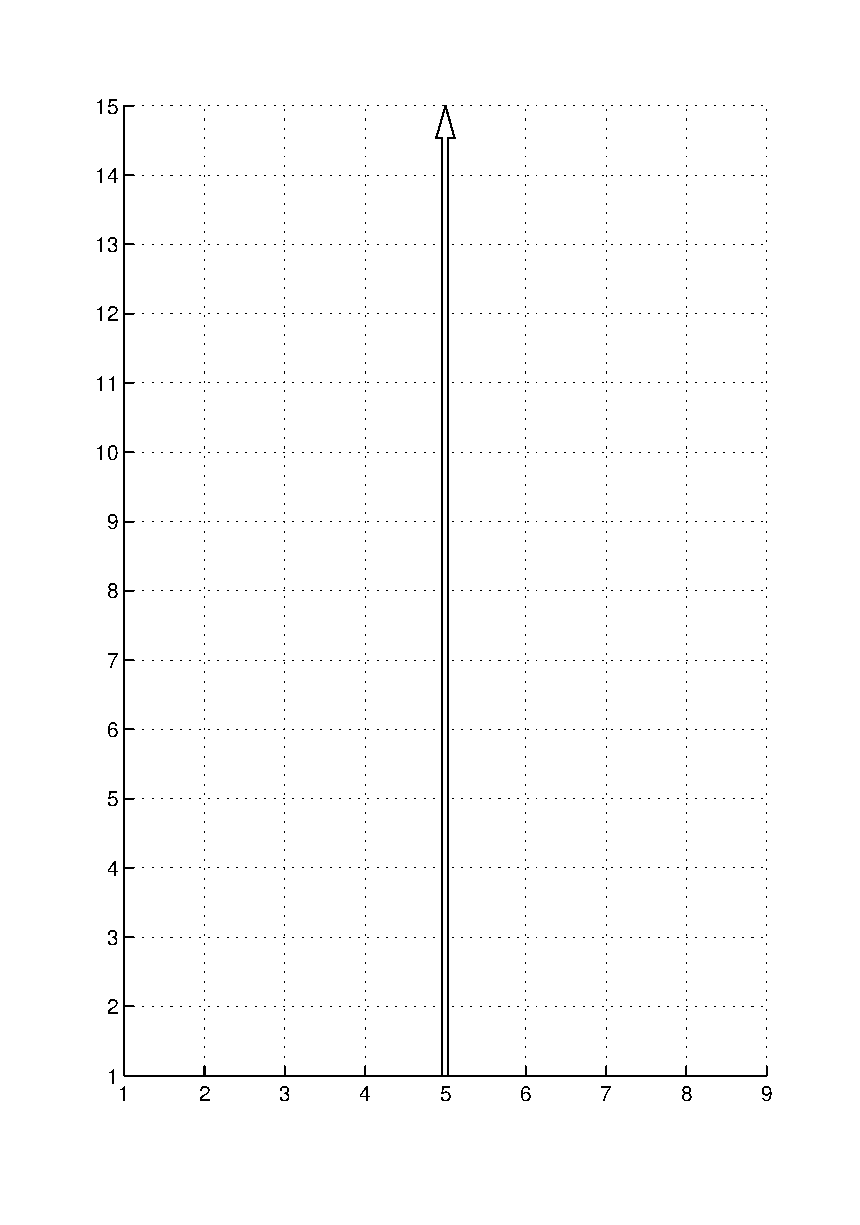
\includegraphics[width=1.7in, height= 2.975in, viewport = 10 50 375 550, clip]{Chapter_2_Figures/path1.eps} \label{Figure: path1.eps}} 
    \subfigure[User trajectory 2.]{\includegraphics[width=1.7in, height= 3.1in, viewport = 10 47 375 550, clip]{Chapter_2_Figures/path2.eps} \label{Figure: path2.eps}} 
    \subfigure[User trajectory 3.]{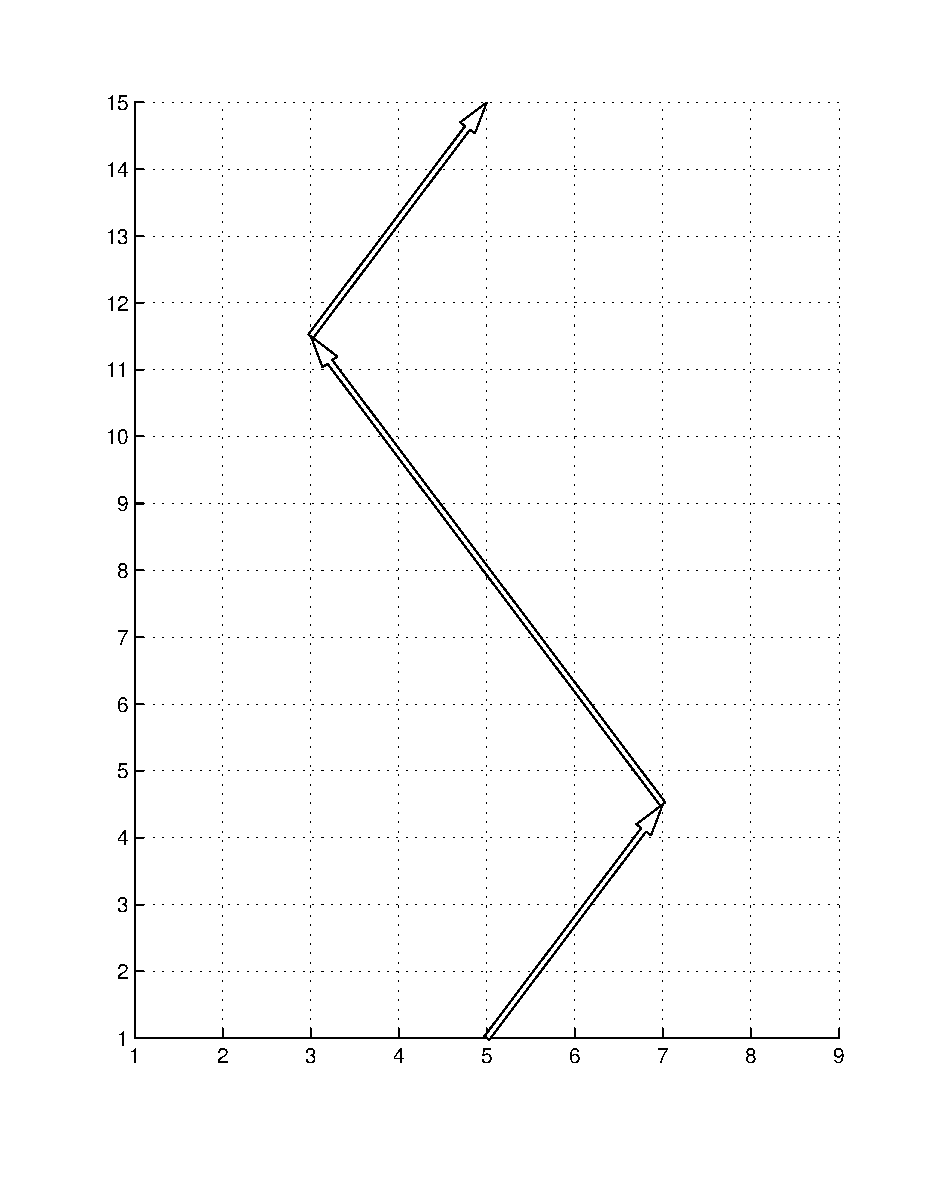
\includegraphics[width=1.7in, height= 3.1in, viewport = 10 47 400 550, clip]{Chapter_2_Figures/path3.eps} \label{Figure: path3.eps}}
\caption{RFID grid with different user trajectories.}
\label{Figure: path123.eps}
\end{figure}
\clearpage

\begin{figure}
\centering
    \subfigure[User trajectory 1.]{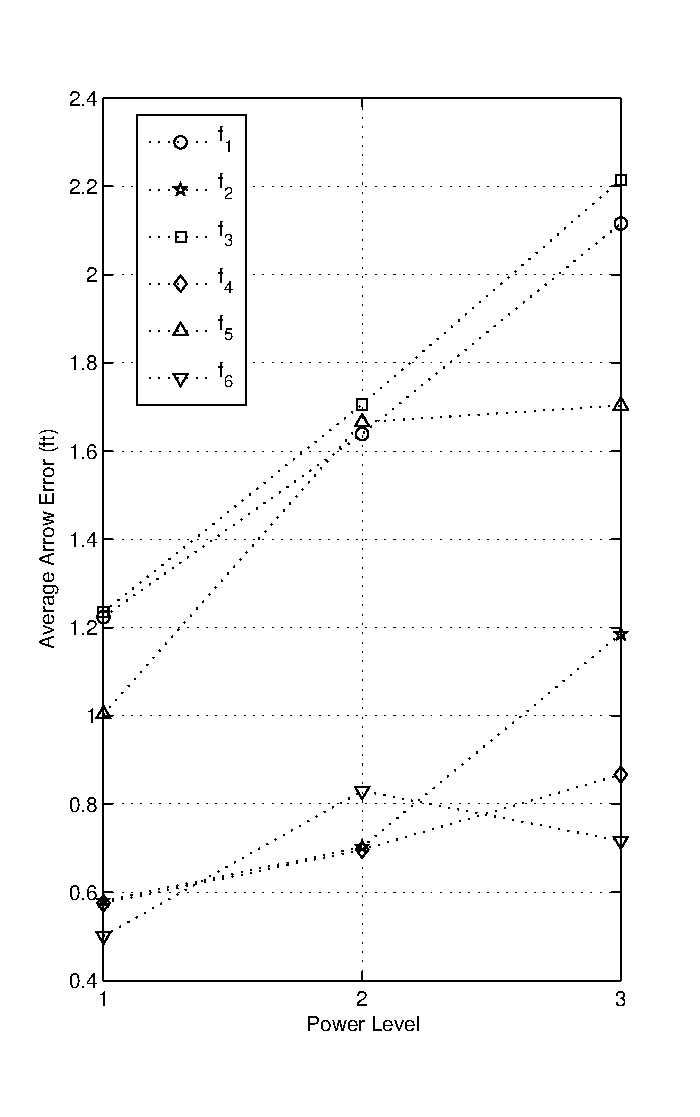
\includegraphics[width= 1.7in, height= 3in, viewport = 10 20 300 500, clip]{Chapter_2_Figures/path1_error.eps} } 
    \subfigure[User trajectory 2.]{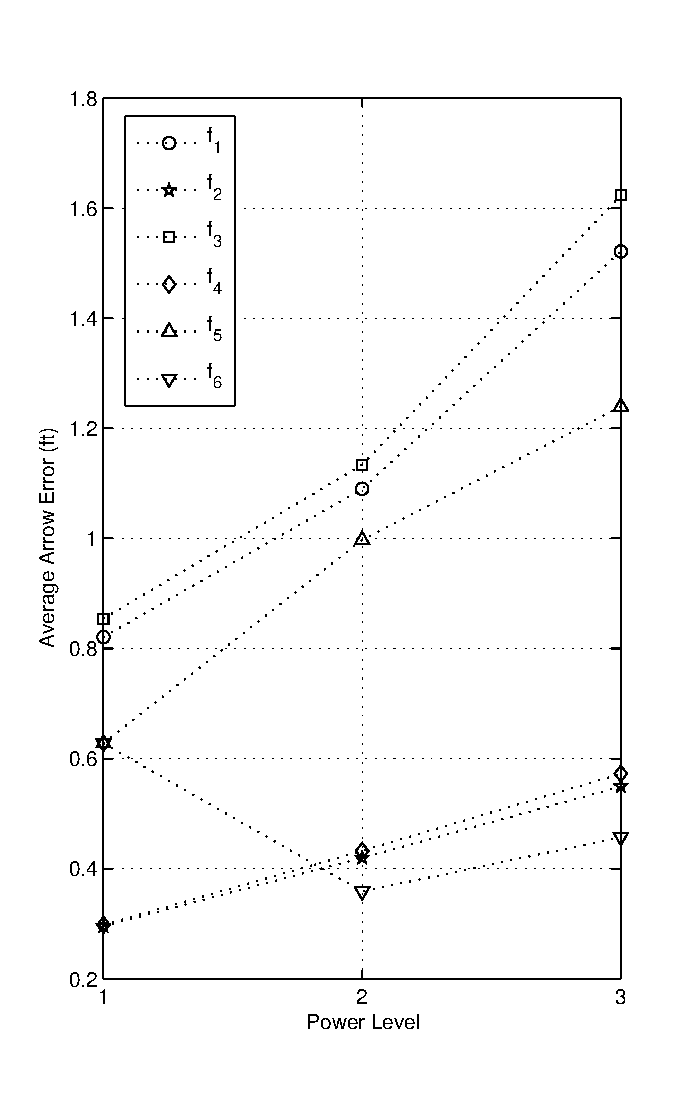
\includegraphics[width= 1.7in, height= 3in, viewport = 10 20 300 500, clip]{Chapter_2_Figures/path2_error.eps} } 
    \subfigure[User trajectory 3.]{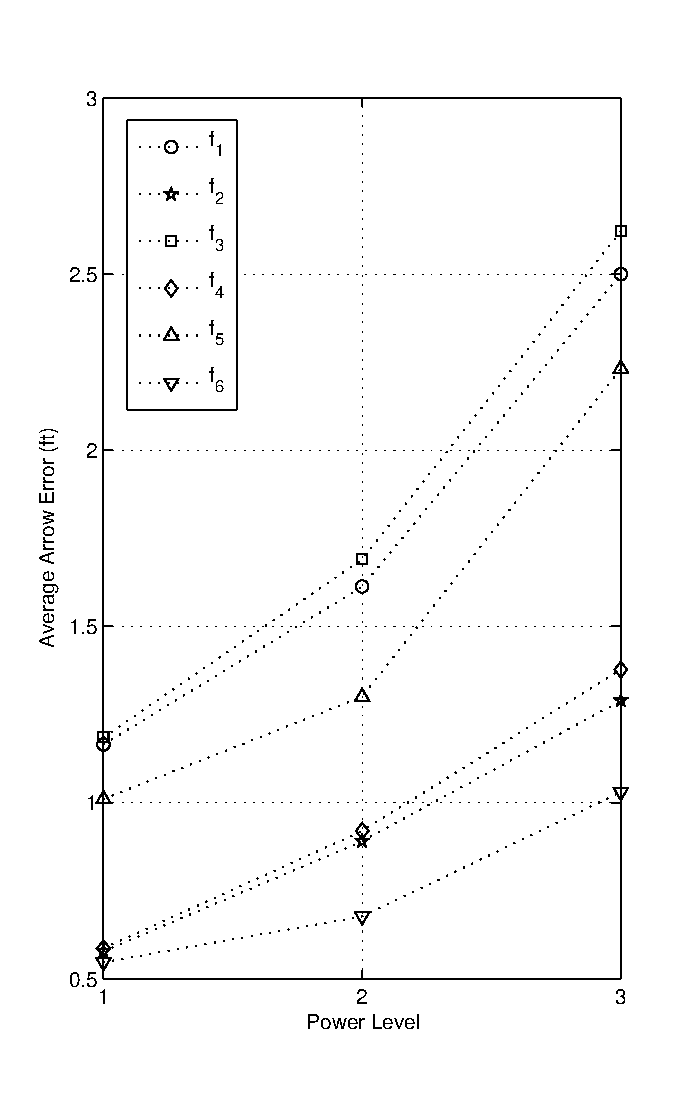
\includegraphics[width= 1.7in, height= 3in, viewport = 10 20 300 500, clip]{Chapter_2_Figures/path3_error.eps} }
\caption{Average weight-normalized arrow error.}
\label{Figure: path123_error.eps}
\end{figure}
\begin{figure}
\centering
    \subfigure[User trajectory 1.]{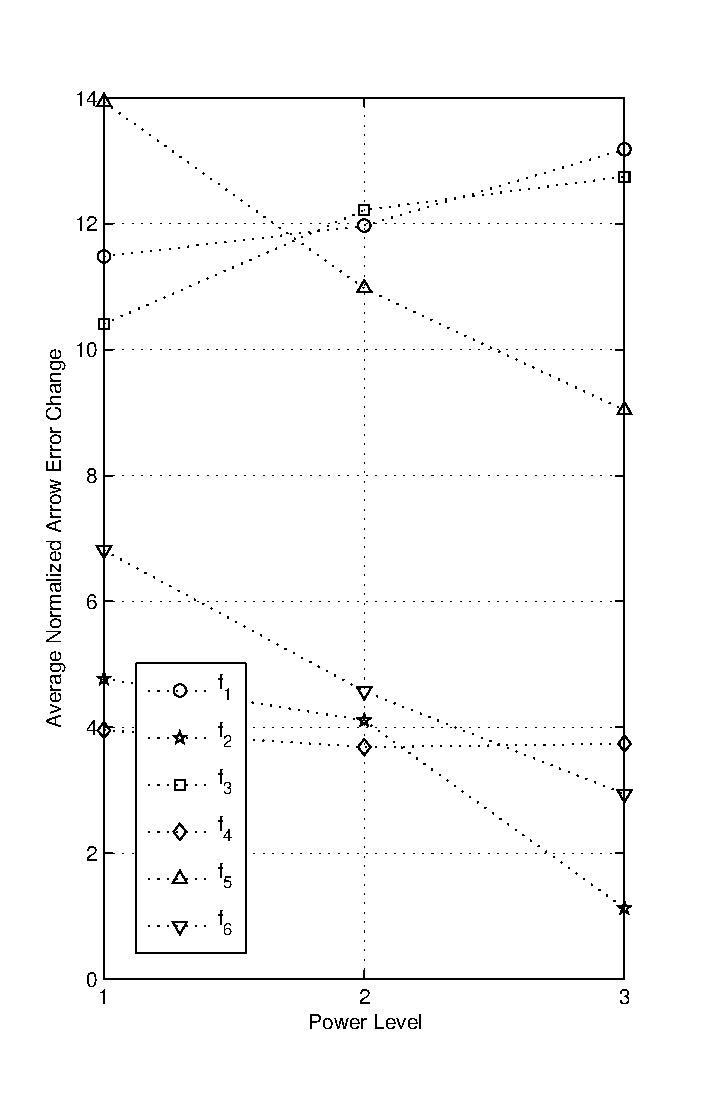
\includegraphics[width= 1.7in, height= 3in, viewport = 5 20 300 500, clip]
{Chapter_2_Figures/path1_change.eps} } 
    \subfigure[User trajectory 2.]{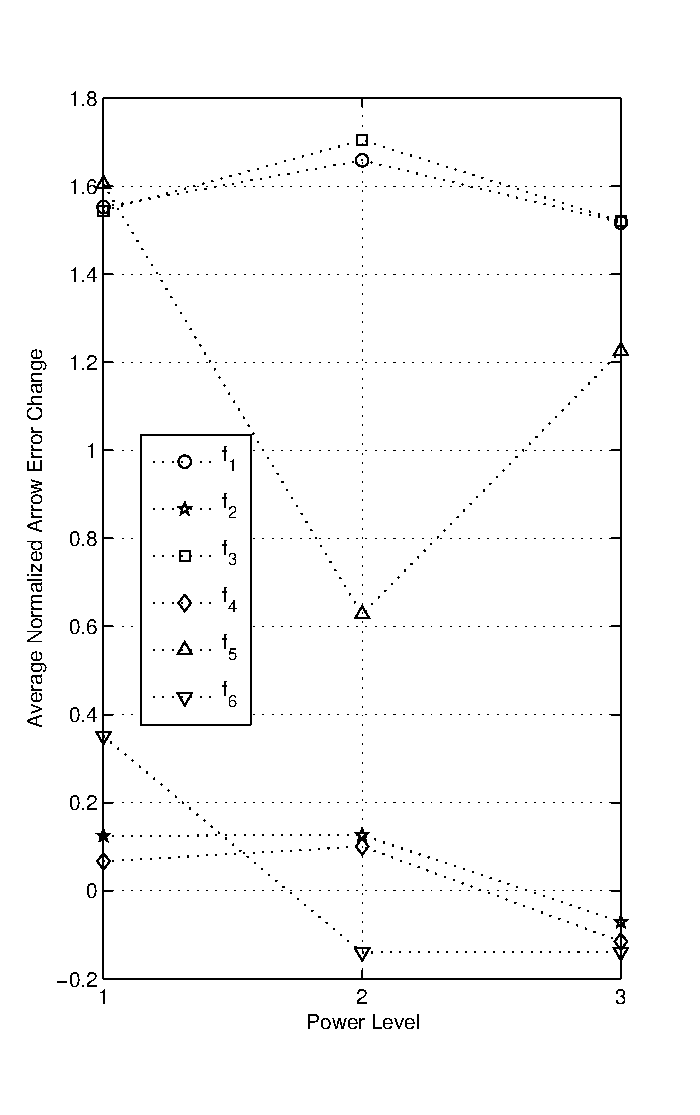
\includegraphics[width= 1.7in, height= 3in, viewport = 5 20 300 500, clip]
{Chapter_2_Figures/path2_change.eps}}
    \subfigure[User trajectory 3.]{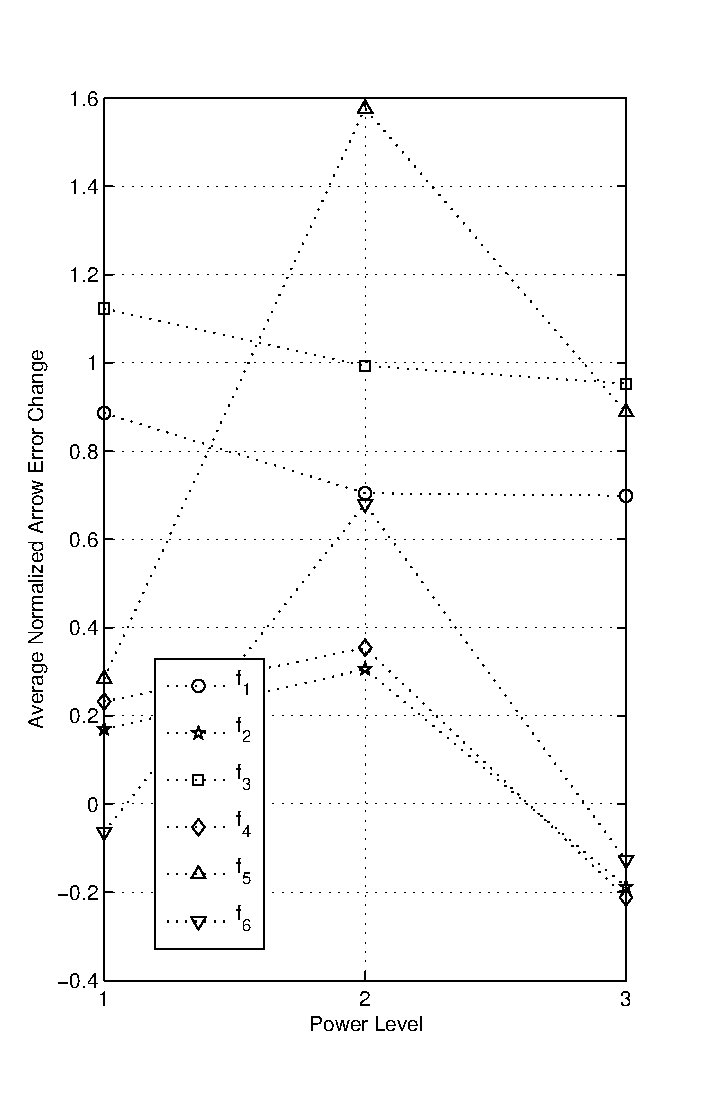
\includegraphics[width= 1.7in, height= 3in, viewport = 5 20 300 500, clip]
{Chapter_2_Figures/path3_change.eps}}
\caption{Average weight-normalized arrow error change.}
\label{Figure: path123_change.eps}
\end{figure}
\clearpage

\begin{figure}
\centering
    \subfigure[User trajectory 1.]{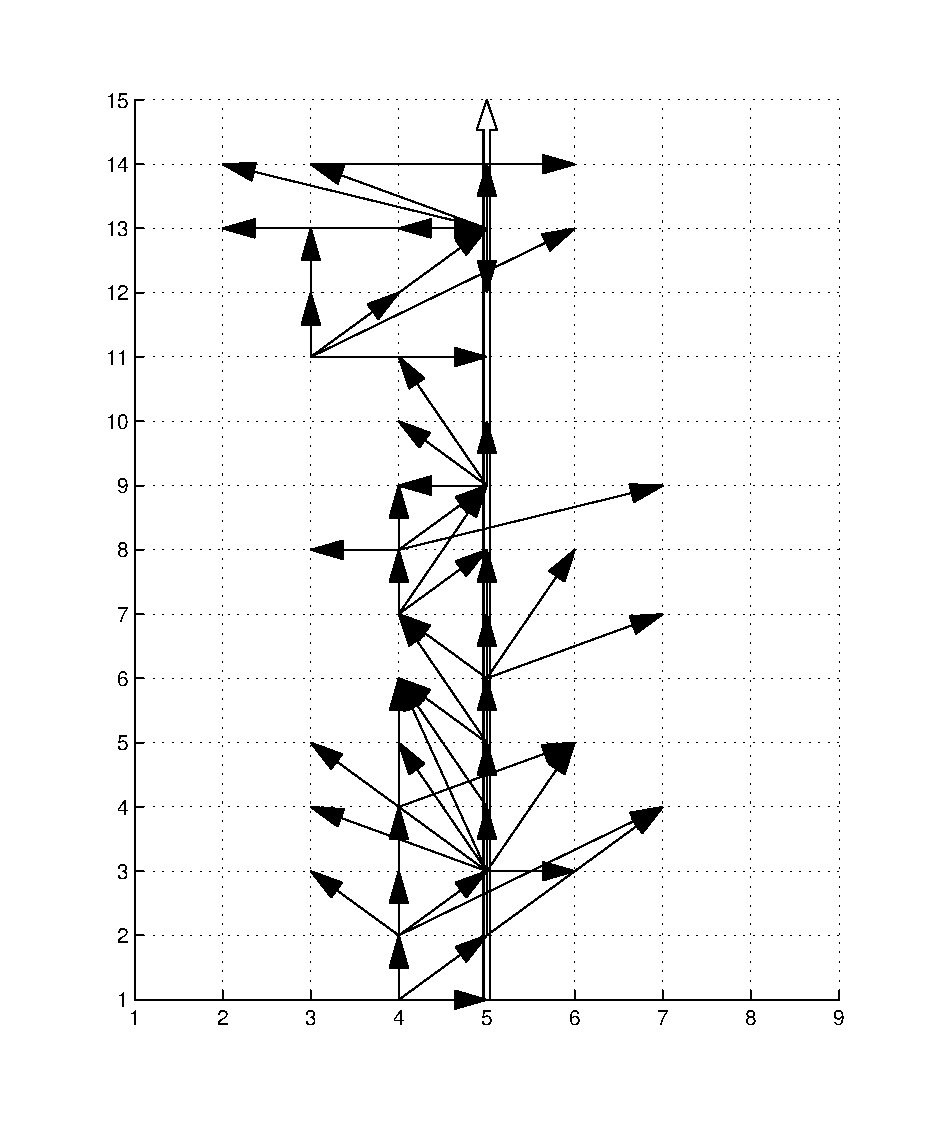
\includegraphics[width= 1.7in, height= 3in, viewport = 45 20 400 500, clip]{Chapter_2_Figures/old_to_new_path1_rf270.eps}} 
    \subfigure[User trajectory 2.]{\includegraphics[width= 1.7in, height= 3in, viewport = 45 20 400 500, clip]{Chapter_2_Figures/old_to_new_path2_rf270.eps}} 
    \subfigure[User trajectory 3.]{\includegraphics[width= 1.7in, height= 3in, viewport = 45 20 400 500, clip]{Chapter_2_Figures/old_to_new_path3_rf270.eps}} 
\caption{Arrow field with $\mathbf{d}^{\left(new\right)}$ from one experiment run.  Antenna power = $P_2$.}
\label{Figure: old_to_new_path123_rf270.eps}
\end{figure}
\begin{figure}
\centering
    \subfigure[User trajectory 1.]{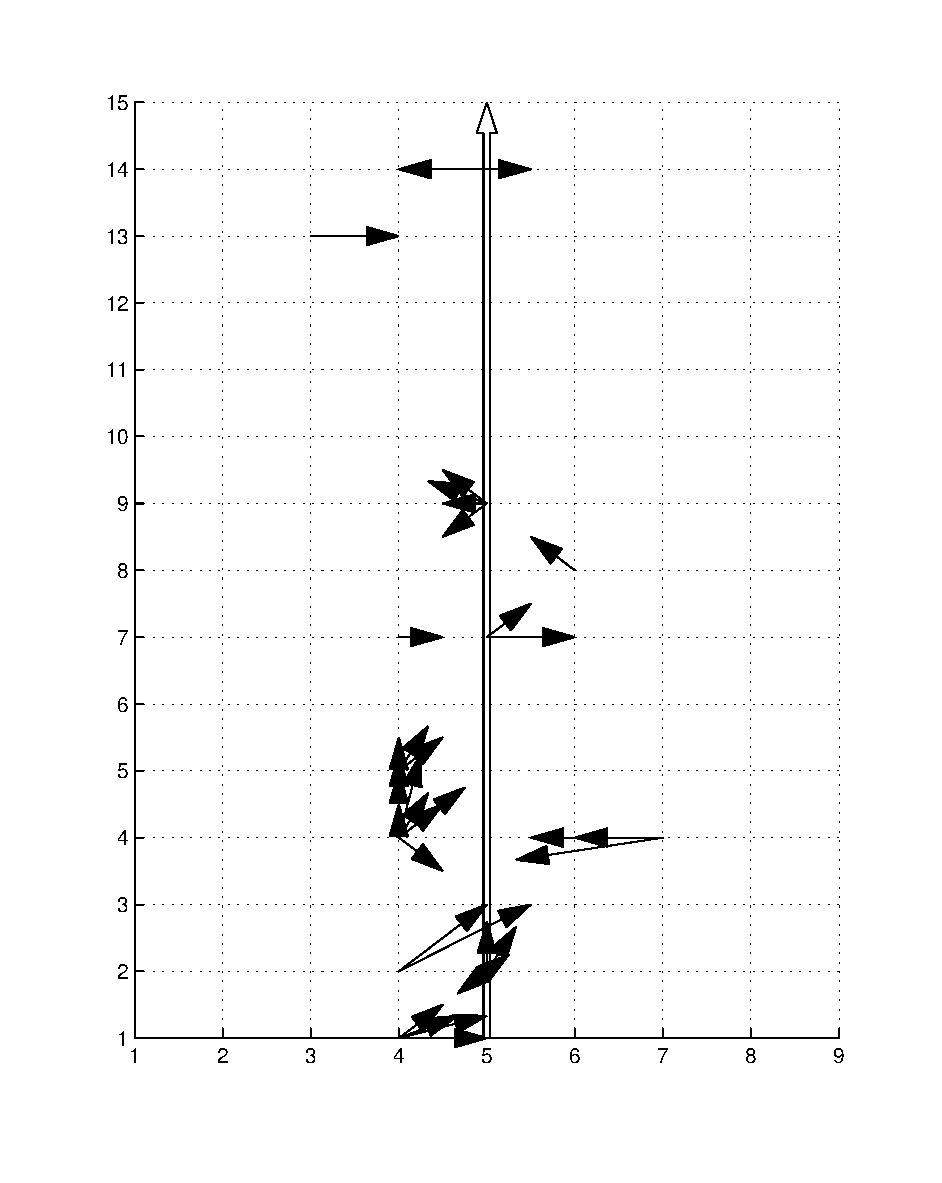
\includegraphics[width= 1.7in, height= 3in, viewport = 45 20 400 515, clip]{Chapter_2_Figures/old_to_centroid_path1_rf250.eps}} 
    \subfigure[User trajectory 2.]{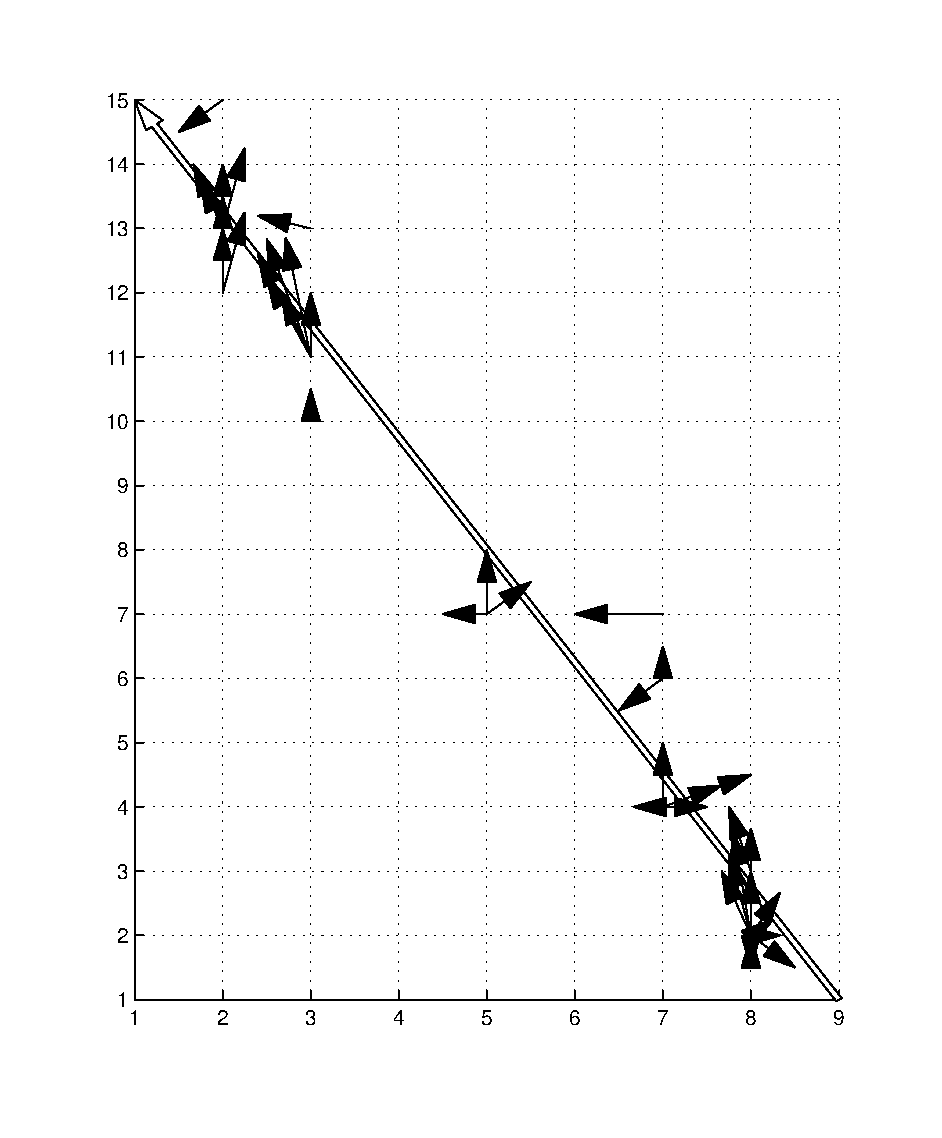
\includegraphics[width= 1.7in, height= 3.04in, viewport = 45 20 400 500, clip]{Chapter_2_Figures/old_to_centroid_path2_rf250.eps}} 
    \subfigure[User trajectory 3.]{\includegraphics[width= 1.7in, height= 3in, viewport = 45 20 400 515, clip]{Chapter_2_Figures/old_to_centroid_path3_rf250.eps}} 
\caption{Arrow field with $\mathbf{d}^{\left(cen\right)}$ from one experiment run.  Antenna power = $P_1$.}
\label{Figure: old_to_centroid_path123_rf250.eps}
\end{figure}
\clearpage

\begin{figure}
\centering
    \subfigure[User trajectory 1.]{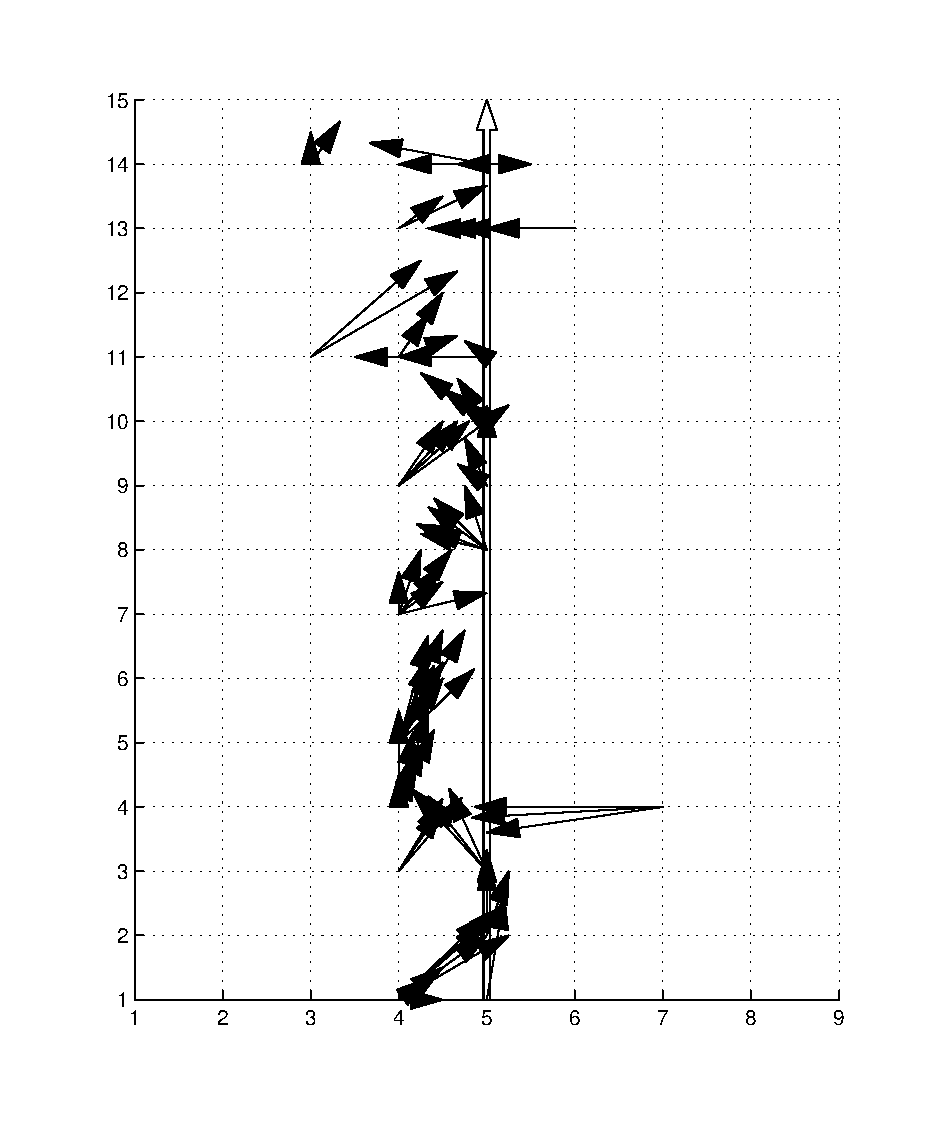
\includegraphics[width= 1.7in, height= 3in, viewport = 45 20 400 500, clip]{Chapter_2_Figures/old_to_centroid_path1_rf270.eps}} 
    \subfigure[User trajectory 2.]{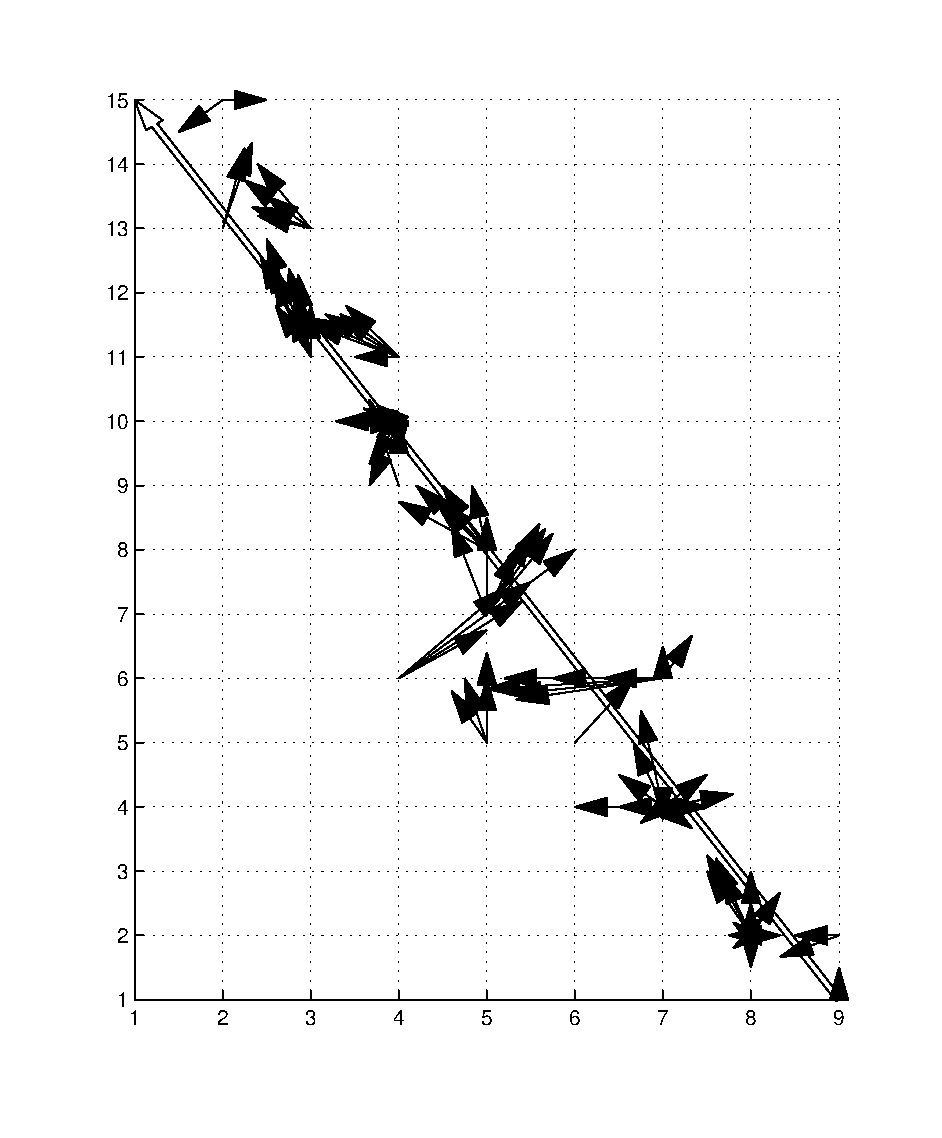
\includegraphics[width= 1.7in, height= 3in, viewport = 45 20 400 500, clip]{Chapter_2_Figures/old_to_centroid_path2_rf270.eps}} 
    \subfigure[User trajectory 3.]{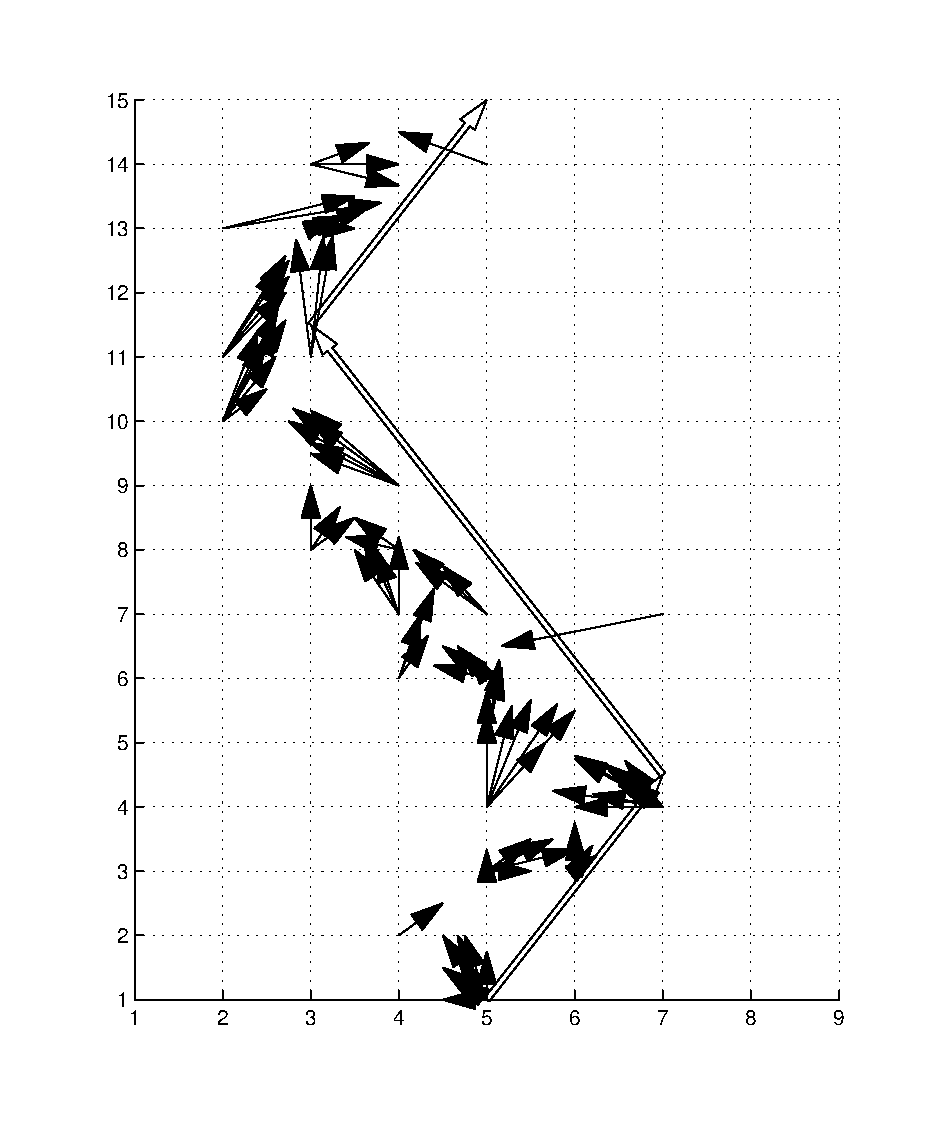
\includegraphics[width= 1.7in, height= 3in, viewport = 45 20 400 500, clip]{Chapter_2_Figures/old_to_centroid_path3_rf270.eps}} 
\caption{Arrow field with $\mathbf{d}^{\left(cen\right)}$ from one experiment run.  Antenna power = $P_2$.}
\label{Figure: old_to_centroid_path123_rf270.eps}
\end{figure}
\begin{figure}
\centering
    \subfigure[User trajectory 1.]{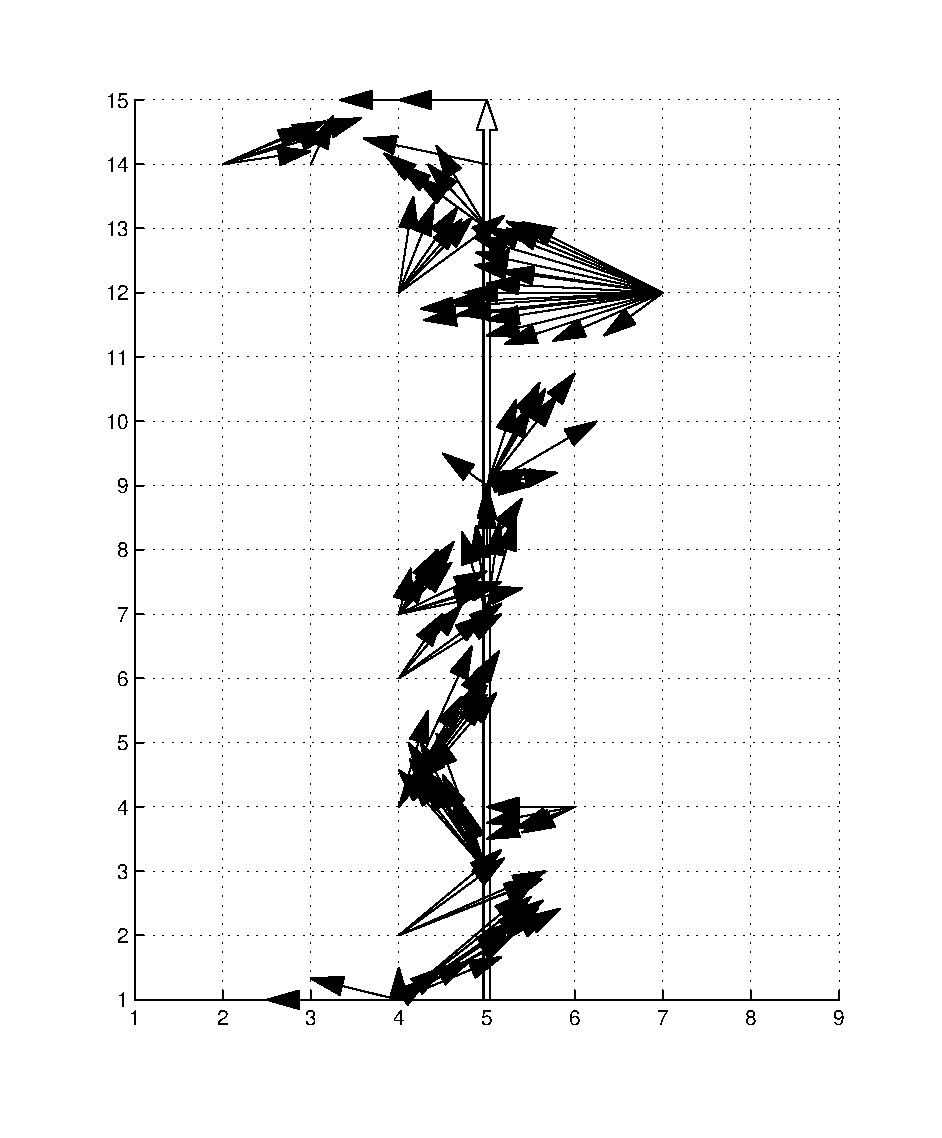
\includegraphics[width= 1.7in, height= 3in, viewport = 45 20 400 500, clip]{Chapter_2_Figures/old_to_centroid_path1_rf290.eps}} 
    \subfigure[User trajectory 2.]{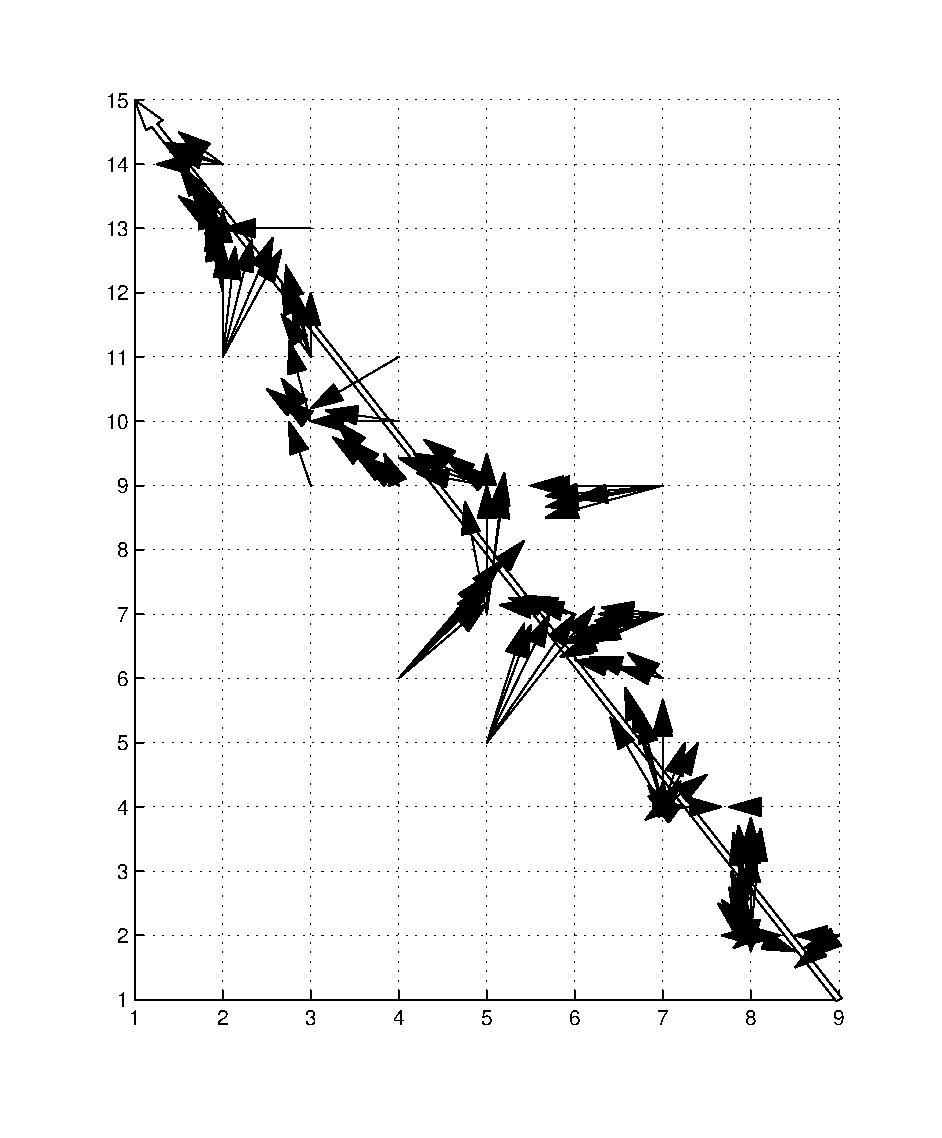
\includegraphics[width= 1.7in, height= 3in, viewport = 45 20 400 500, clip]{Chapter_2_Figures/old_to_centroid_path2_rf290.eps}} 
    \subfigure[User trajectory 3.]{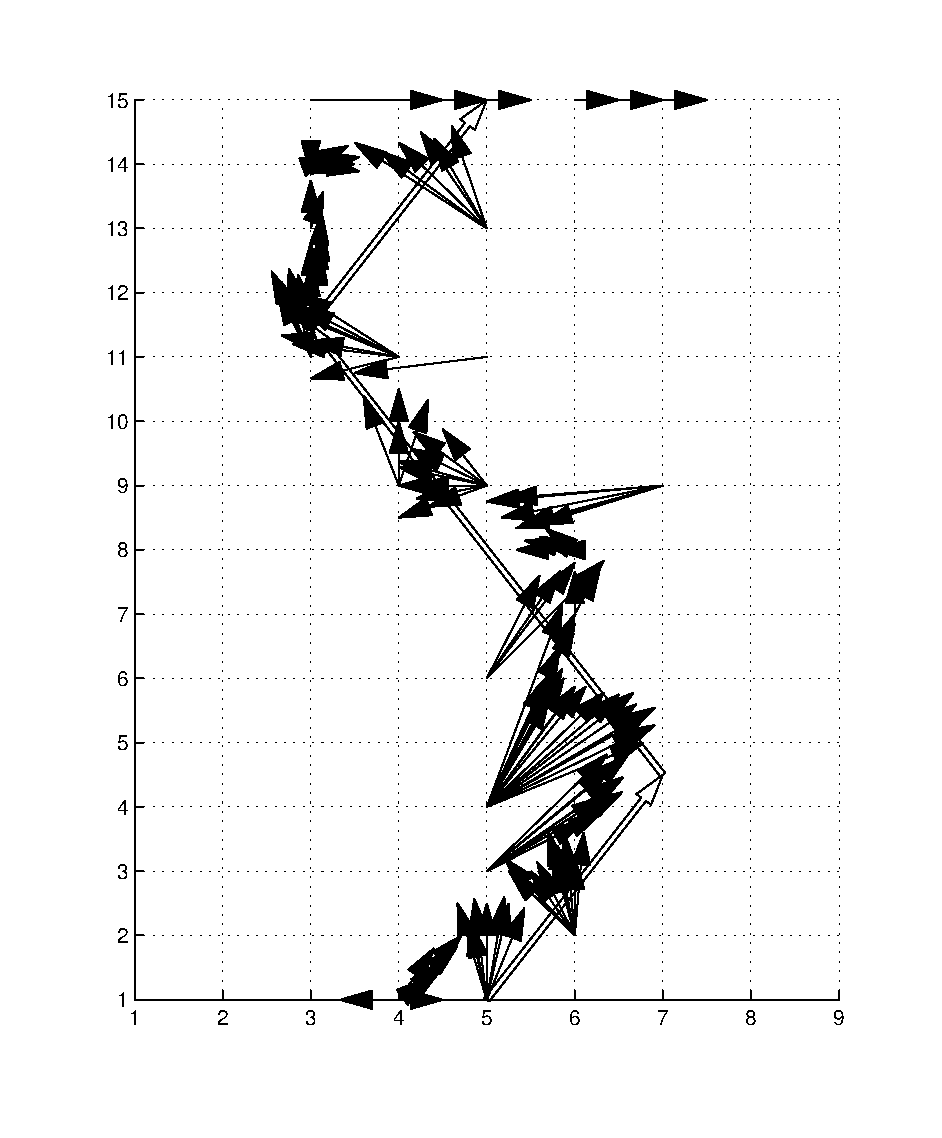
\includegraphics[width= 1.7in, height= 3in, viewport = 45 20 400 500, clip]{Chapter_2_Figures/old_to_centroid_path3_rf290.eps}} 
\caption{Arrow field with $\mathbf{d}^{\left(cen\right)}$ from one experiment run.  Antenna power = $P_3$.}
\label{Figure: old_to_centroid_path123_rf290.eps}
\end{figure}
\clearpage

\begin{figure}
\centering
    \subfigure[User trajectory 1.]{\includegraphics[width= 1.7in, height= 3in, viewport = 45 20 400 500, clip]{Chapter_2_Figures/all_to_new_path1_rf290.eps}}
    \subfigure[User trajectory 2.]{\includegraphics[width= 1.7in, height= 3in, viewport = 45 20 400 500, clip]{Chapter_2_Figures/all_to_new_path2_rf290.eps}}
    \subfigure[User trajectory 3.]{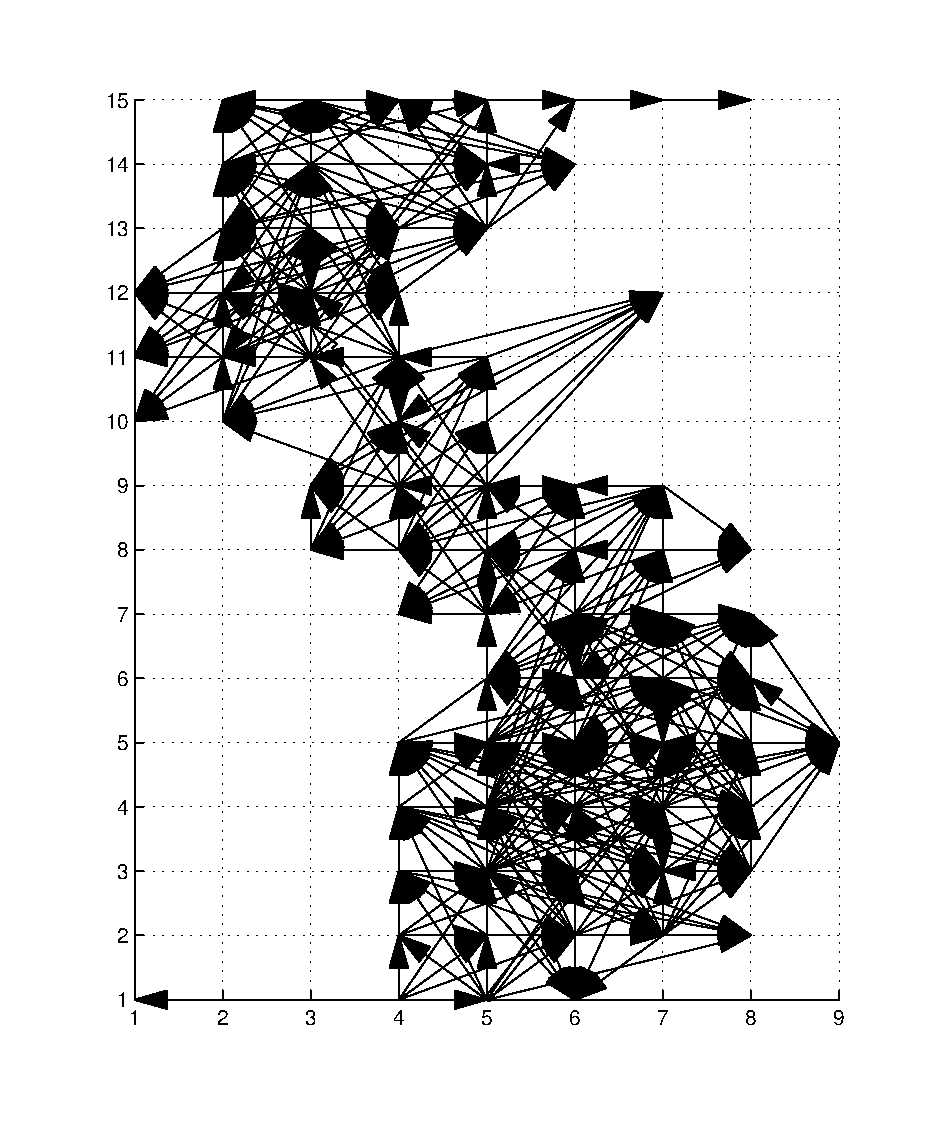
\includegraphics[width= 1.7in, height= 3in, viewport = 45 20 400 500, clip]{Chapter_2_Figures/all_to_new_path3_rf290.eps}}
\caption{Arrow field with $\mathbf{d}^{\left(sar,new\right)}$ from one experiment run.  Antenna power = $P_3$.}
\label{Figure: all_to_new_path123_rf290.eps}
\end{figure}
\begin{figure}
\centering
    \subfigure[User trajectory 1.]{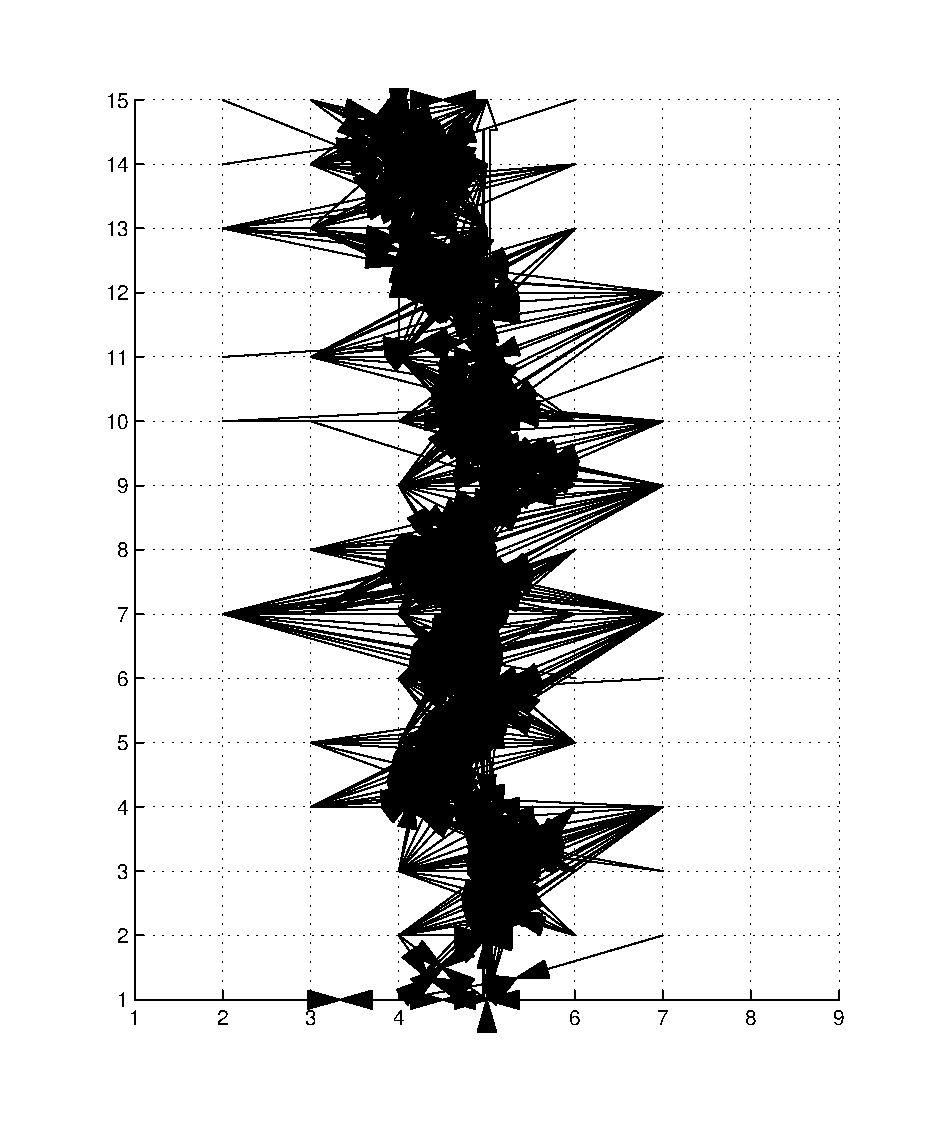
\includegraphics[width= 1.7in, height=3in, viewport = 45 20 400 500, clip]{Chapter_2_Figures/all_to_centroid_path1_rf290.eps}}
    \subfigure[User trajectory 2.]{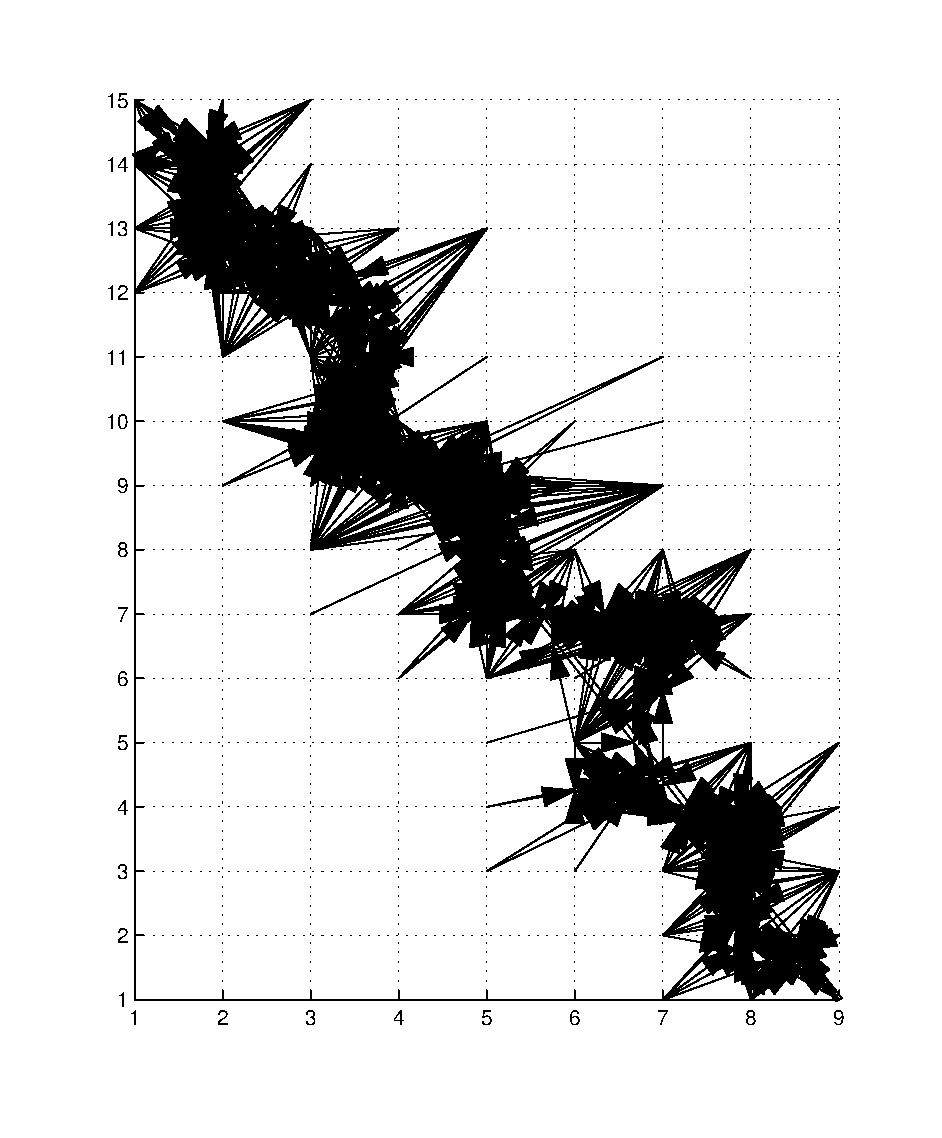
\includegraphics[width= 1.7in, height=3in, viewport = 45 20 400 500, clip]{Chapter_2_Figures/all_to_centroid_path2_rf290.eps}}
    \subfigure[User trajectory 3.]{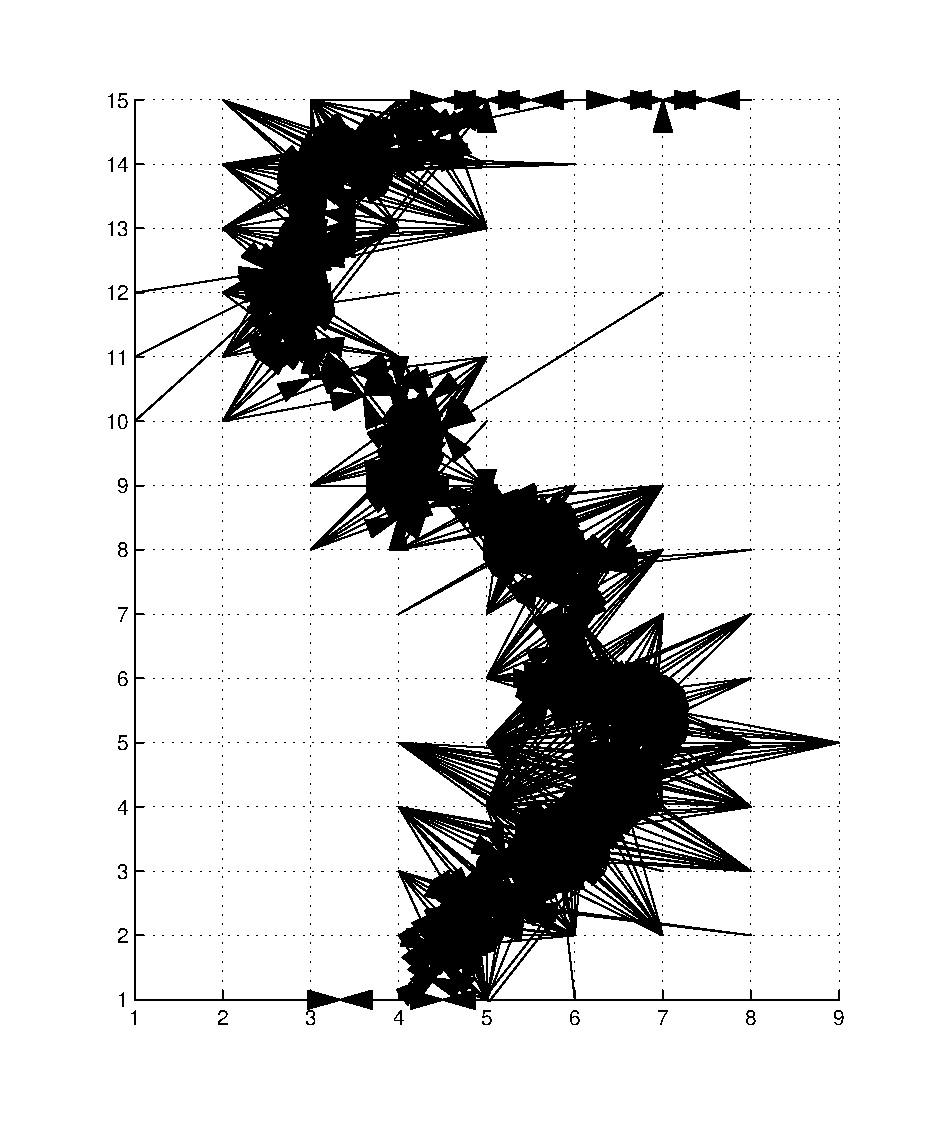
\includegraphics[width= 1.7in, height=3in, viewport = 45 20 400 500, clip]{Chapter_2_Figures/all_to_centroid_path3_rf290.eps}}
\caption{Arrow field with $\mathbf{d}^{\left(sar,cen\right)}$ from one experiment run.  Antenna power = $P_3$.}
\label{Figure: all_to_centroid_path123_rf290.eps}
\end{figure}
\clearpage

\begin{figure}
\centering
	\subfigure[User trajectory 1.]{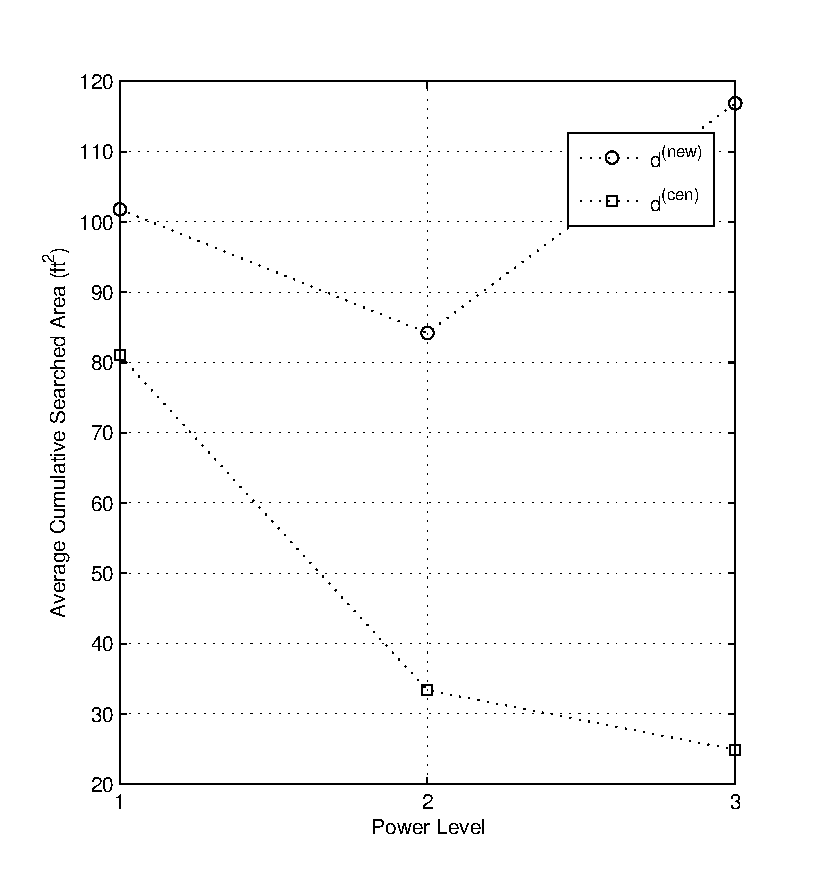
\includegraphics[width= 1.7in, height=3in, viewport = 10 20 350 500, clip]{Chapter_2_Figures/path1_searched_area.eps}}
	\subfigure[User trajectory 2.]{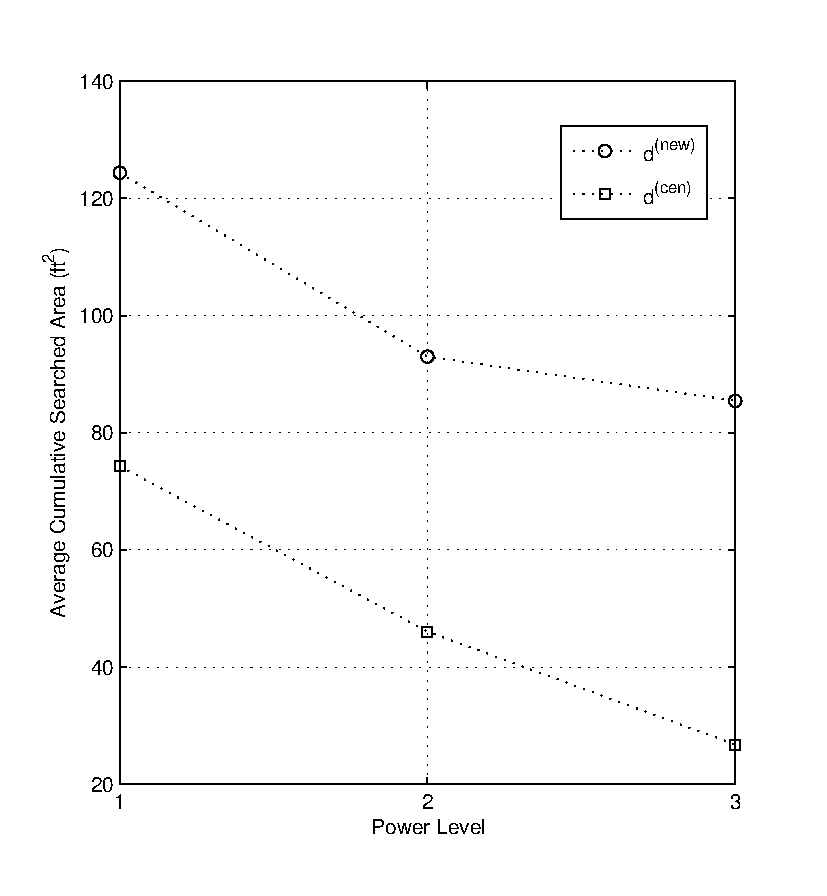
\includegraphics[width= 1.7in, height=3in, viewport = 10 20 350 500, clip]{Chapter_2_Figures/path2_searched_area.eps}}
	\subfigure[User trajectory 3.]{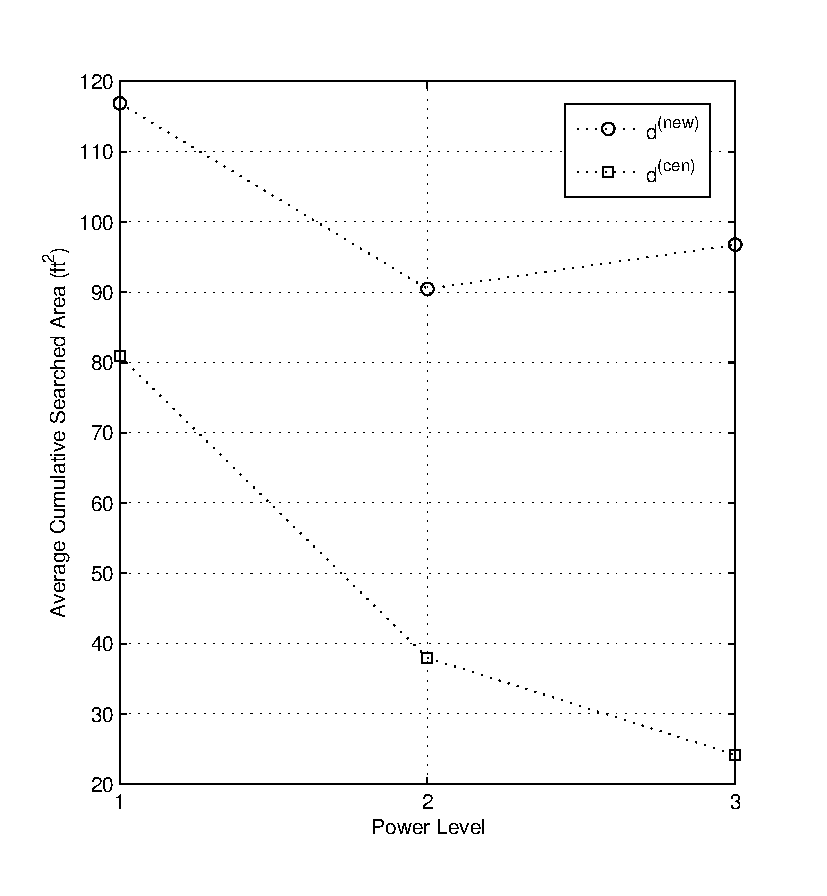
\includegraphics[width= 1.7in, height=3in, viewport = 10 20 350 500, clip]{Chapter_2_Figures/path3_searched_area.eps}}
\caption{Average cumulative searched area.}
\label{Figure: path123_searched_area.eps}
\end{figure}
\begin{figure}
\centering
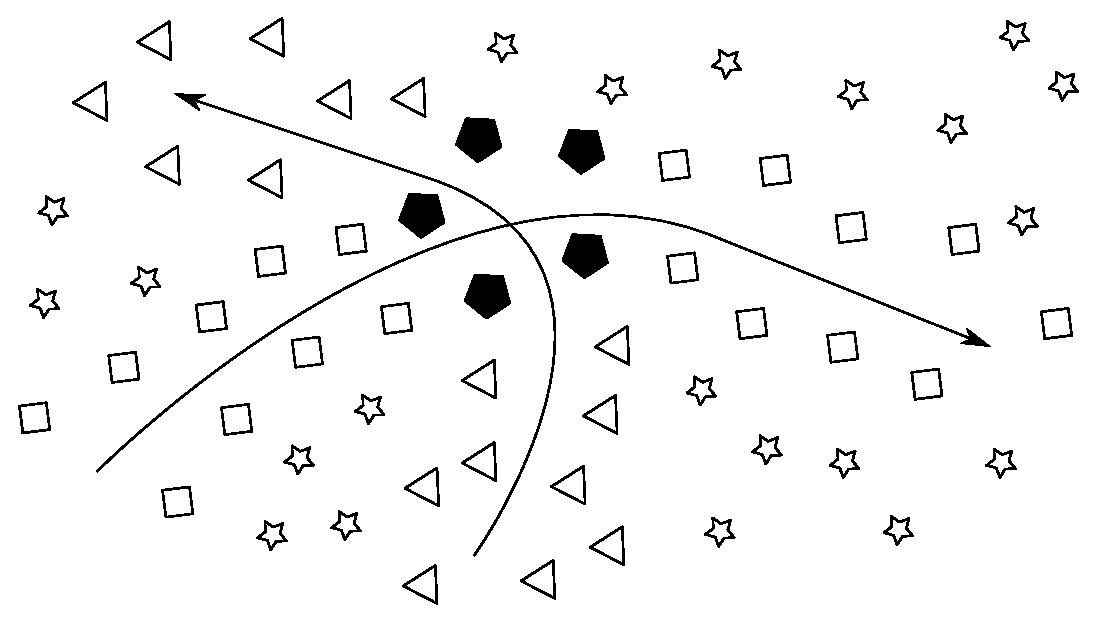
\includegraphics[width=5in]{Chapter_2_Figures/hiker_paths.eps}
\caption{Hiker digital paths stored in RFID tags.}
\label{Figure: hiker_paths.eps}
\end{figure}
\clearpage

\begin{figure}
\centering
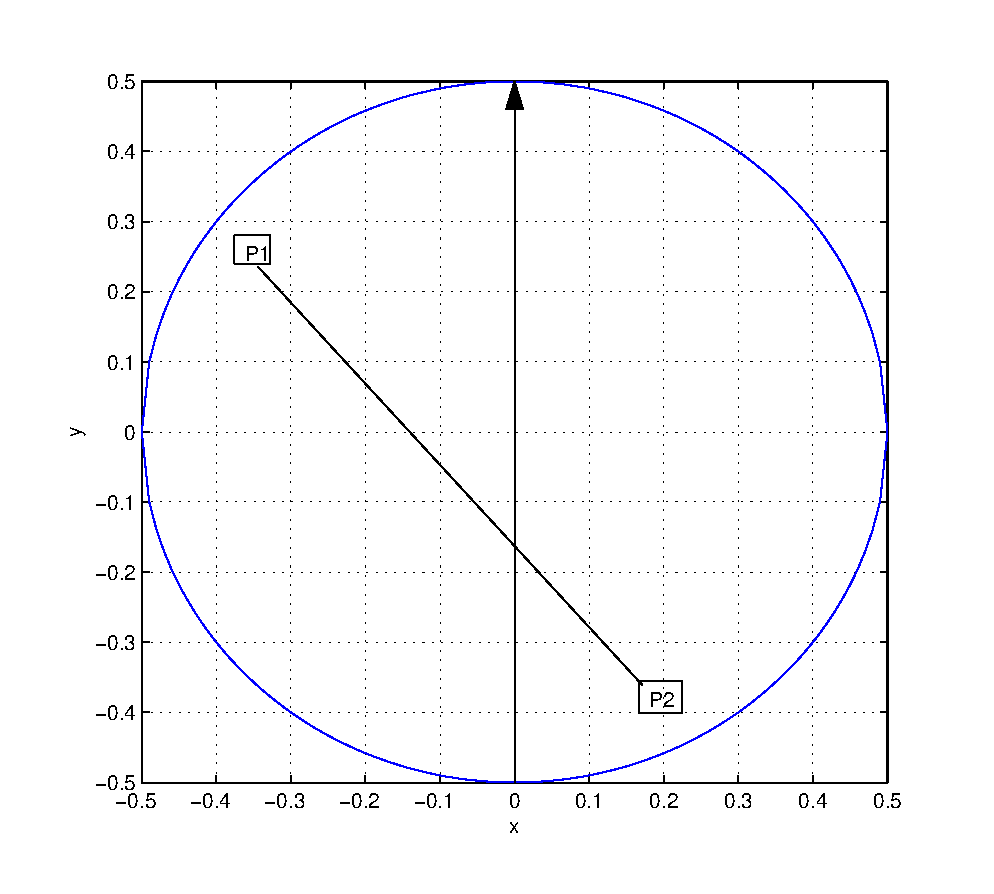
\includegraphics[width=4.5in]{Chapter_2_Figures/hiker_circle.eps}
\caption{The field where hikers can move.  $L = 1$.  The original hiker path is shown by the arrow.}
\label{Figure: hiker_circle.eps}
\end{figure}
\begin{figure}
\centering
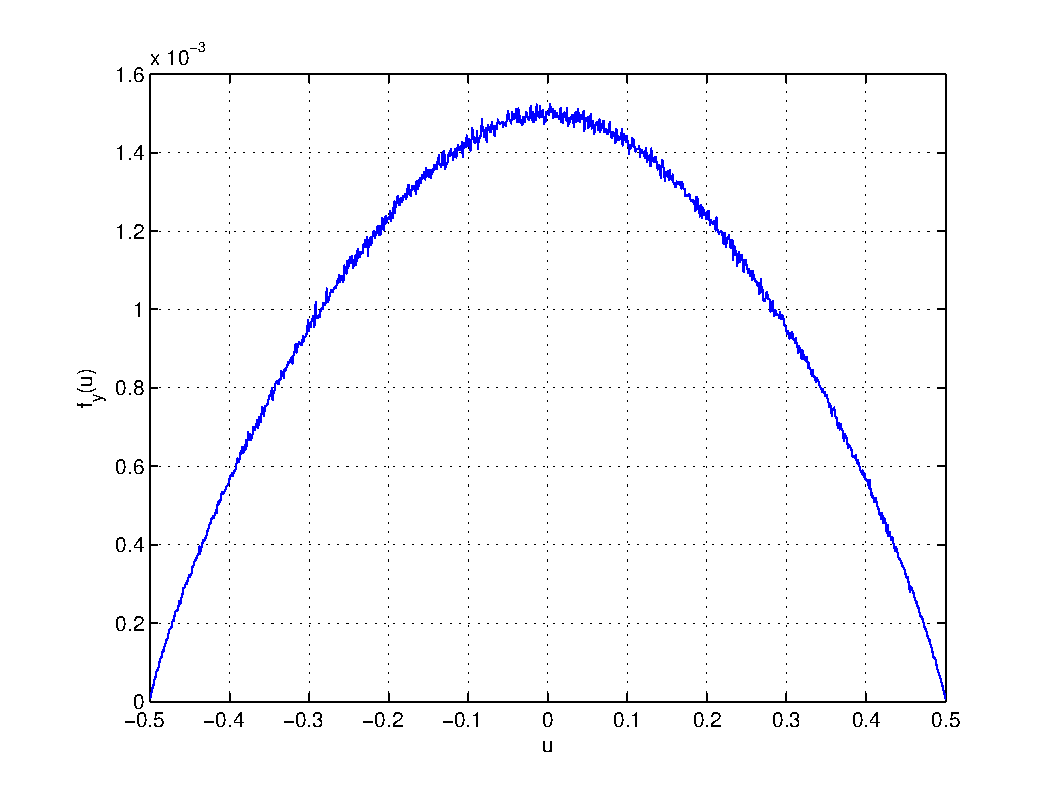
\includegraphics[width=4.5in]{Chapter_2_Figures/hiker_pdf.eps}
\caption{Probability density function of where later hikers intersect $\mathcal{L}$.}
\label{Figure: hiker_pdf.eps}
\end{figure}
\clearpage

\begin{figure}
\centering
\includegraphics[clip=true, viewport=0 280 625 600, width=5in]{Chapter_2_Figures/yosemite_trail.eps}
\caption{Yosemite Valley hiking trail.} 
\label{Figure: yosemite_trail.eps}
\end{figure}
\begin{figure}
\centering
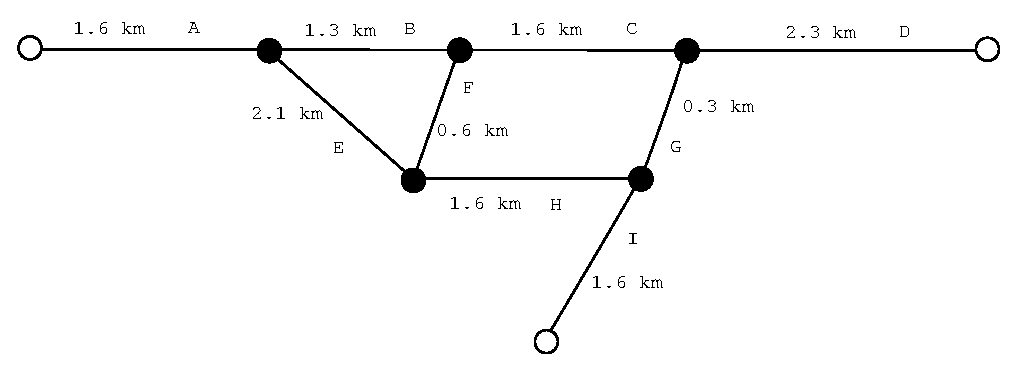
\includegraphics[width=5in]{Chapter_2_Figures/yosemite_sections.eps}
\caption{Yosemite Valley hiking trail sections.}
\label{Figure: yosemite_sections.eps}
\end{figure}
\clearpage

\begin{figure}
\centering
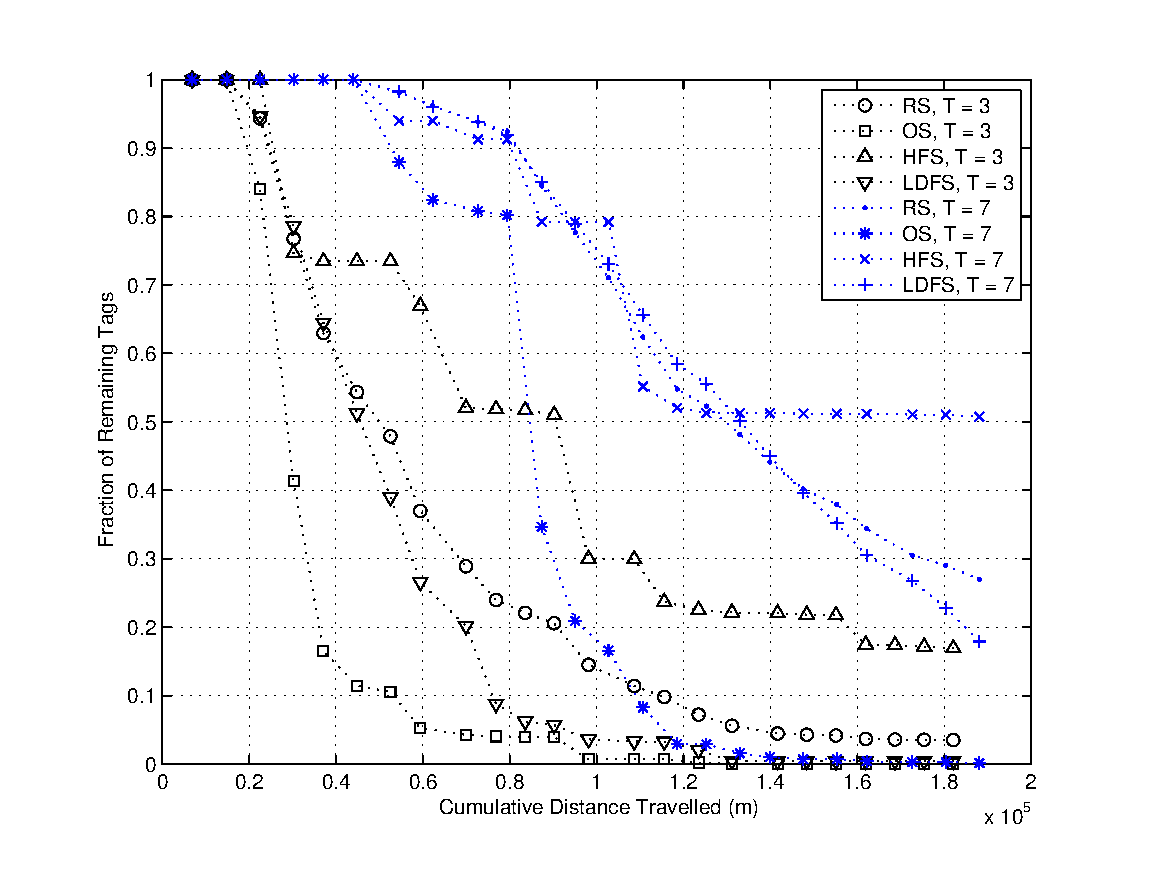
\includegraphics[width=5in]{Chapter_2_Figures/frac_dense01.eps}
\caption{Fraction of remaining tags with (ID, SN) pairs of the first hiker. $\rho = 1$ tag/m$^2$.}
\label{Figure: frac_dense01.eps}
\end{figure}
\begin{figure}
\centering
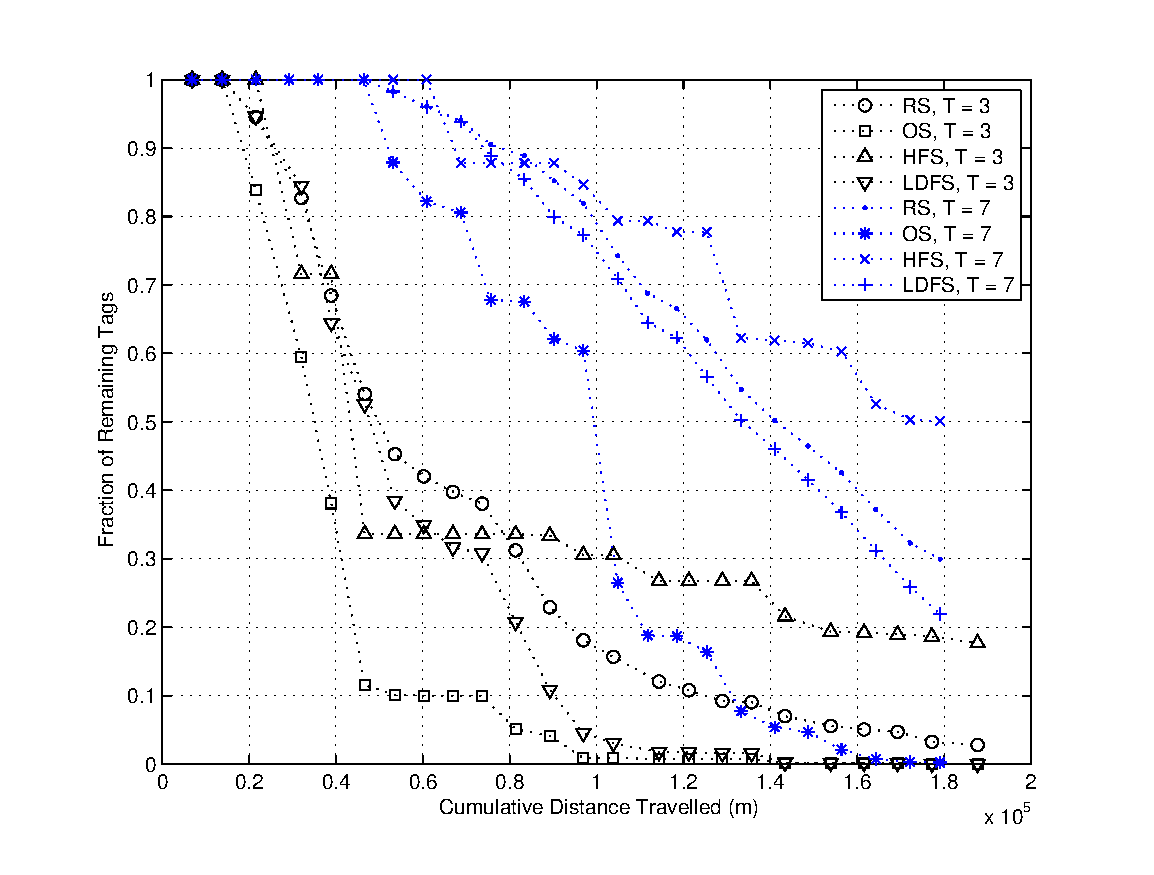
\includegraphics[width=5in]{Chapter_2_Figures/frac_dense05.eps}
\caption{Fraction of remaining tags with (ID, SN) pairs of the first hiker. $\rho = 5$ tags/m$^2$.}
\label{Figure: frac_dense05.eps}
\end{figure}
\clearpage

\begin{figure}
\centering
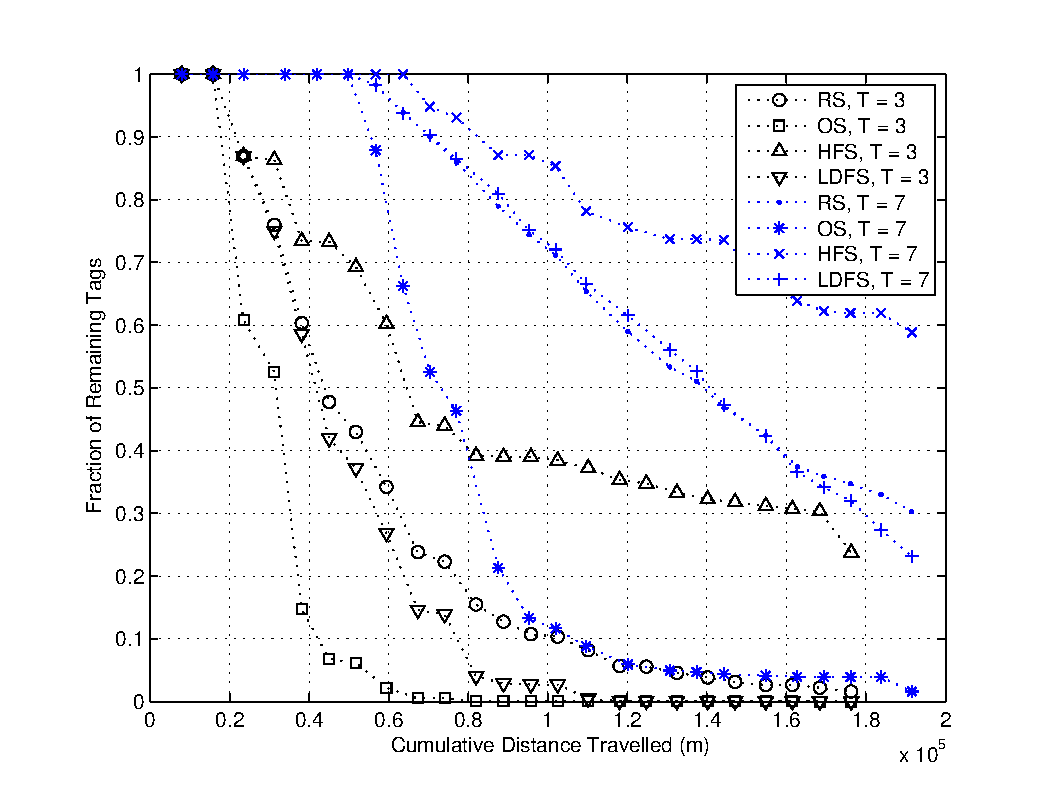
\includegraphics[width=5in]{Chapter_2_Figures/frac_dense10.eps}
\caption{Fraction of remaining tags with (ID, SN) pairs of the first hiker. $\rho = 10$ tags/m$^2$.}
\label{Figure: frac_dense10.eps}
\end{figure}
\begin{figure}
\centering
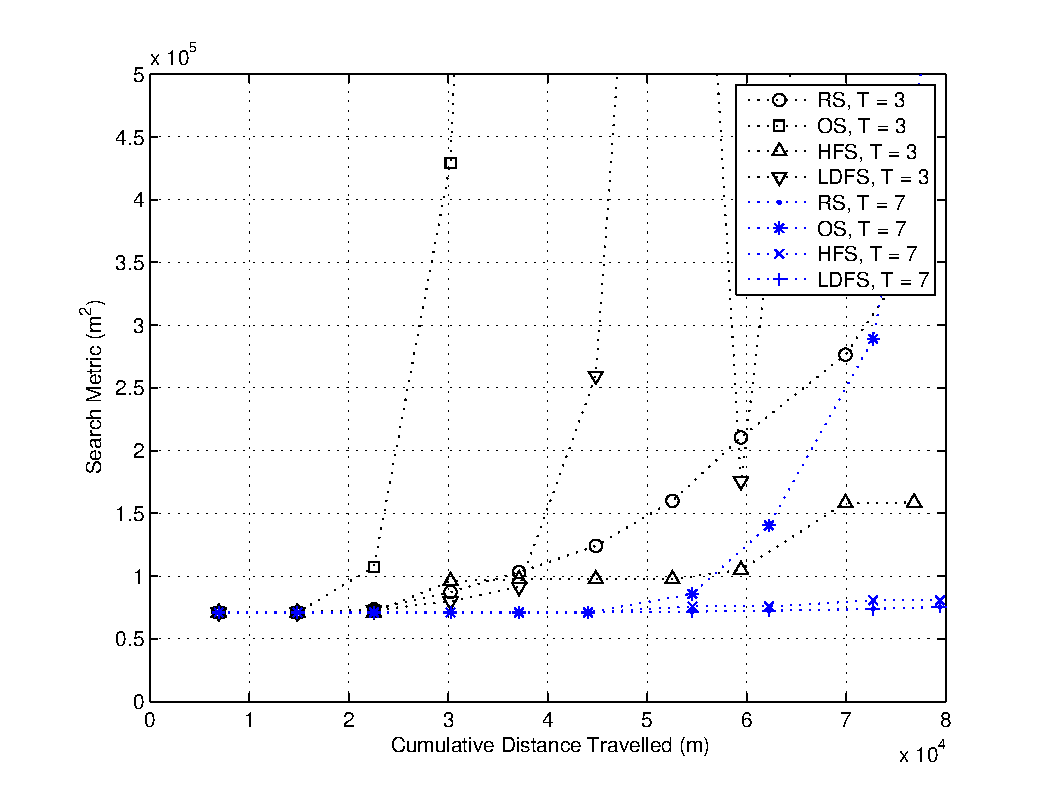
\includegraphics[width=5in]{Chapter_2_Figures/search_dense01.eps}
\caption{Search metric. $\rho = 1$ tag/m$^2$.}
\label{Figure: search_dense01.eps}
\end{figure}
\clearpage

\begin{figure}
\centering
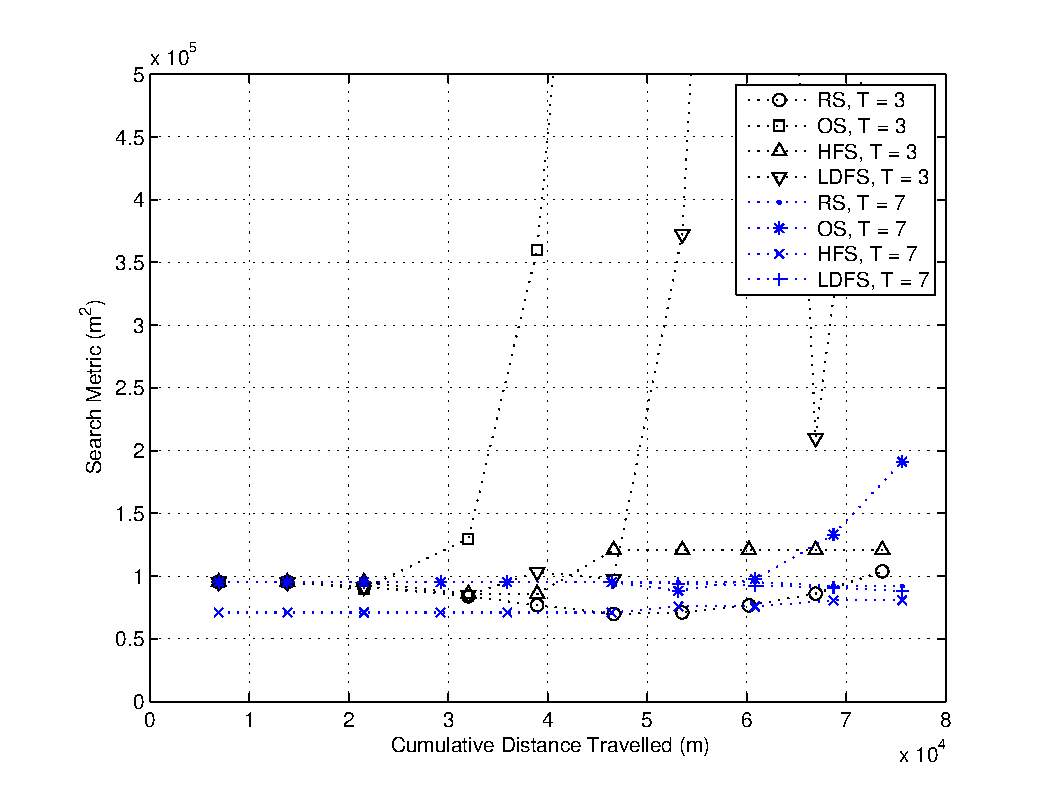
\includegraphics[width=5in]{Chapter_2_Figures/search_dense05.eps}
\caption{Search metric. $\rho = 5$ tags/m$^2$.}
\label{Figure: search_dense05.eps}
\end{figure}
\begin{figure}
\centering
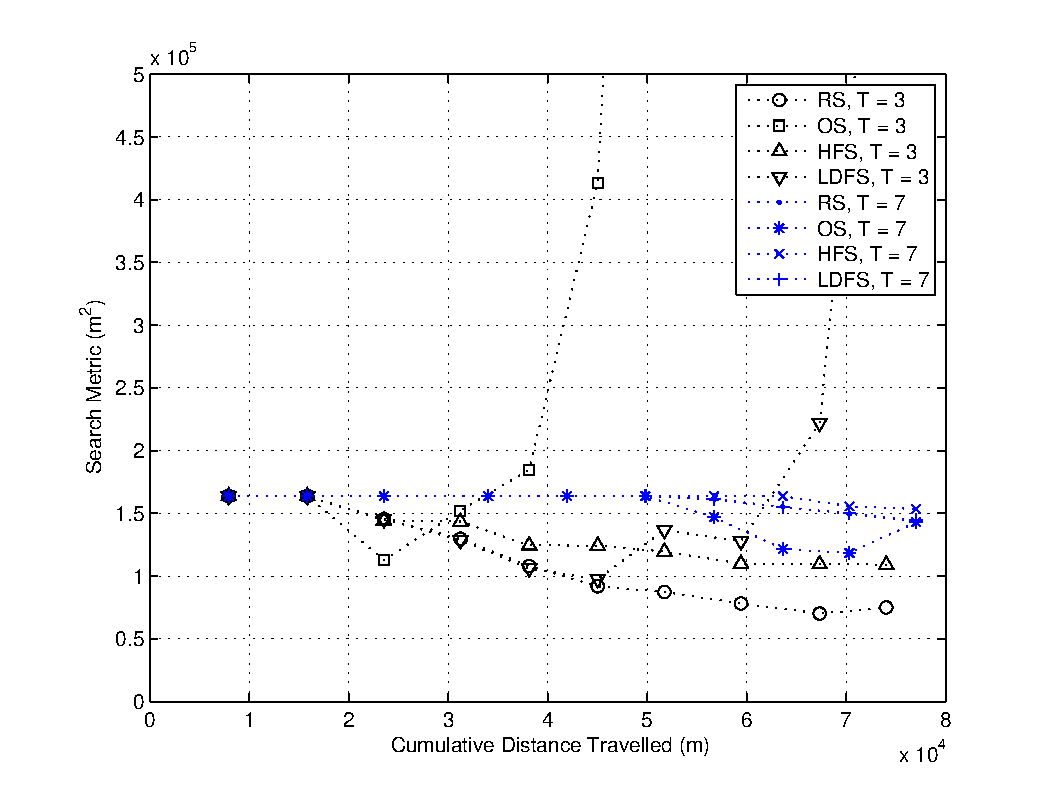
\includegraphics[width=5in]{Chapter_2_Figures/search_dense10.eps}
\caption{Search metric. $\rho = 10$ tags/m$^2$.}
\label{Figure: search_dense10.eps}
\end{figure}
\clearpage

\begin{table}
\caption{(ID, SN) pairs in tag, Cases 1 to 4.}
\label{Table: (ID, SN) pairs in tag, Cases 1 to 4.}
\begin{center}
\begin{tabular}{|c|c|c|c|c|}
\hline
Before & Case 1 & Case 2 & Case 3 (OS) & Case 4 (RS) \\
\hline
$(2, 13)$     & $(2, 13)$      & $(2, 13)$       & $(21, 24)$   & $(2, 13)$  \\
$(100, 12)$ & $(100, 12)$  & $(100, 12)$   & $(2, 13)$     & $(100, 12)$  \\
$(15, 99)$   & $(15, 99)$    & $(15, 106)$   & $(100, 12)$ & $(15, 99)$ \\
$(41, 6)$     & $(41, 6)$      & $(41, 6)$       & $(15, 99)$   & $(21, 24)$ \\
$(75, 92)$   & $(75, 92)$    & $(75, 92)$     & $(41, 6)$     & $(75, 92)$ \\
                   & $(21, 24)$    &             &             & \\
\hline
\end{tabular}
\end{center}
\end{table}


\begin{table}
\caption{See frequencies.}
\label{Table: See frequencies.}
\begin{center}
\begin{tabular}{|c|c|c|}
\hline
ID & See Frequencies \\
\hline
2 & 8   \\
15 & 65    \\
41 & 50  \\
79 & 43 \\
86 & 5    \\
92 & 72\\
\hline
\end{tabular}
\end{center}
\end{table}

\begin{table}
\caption{Delete frequencies.}
\label{Table: Delete frequencies.}
\begin{center}
\begin{tabular}{|c|c|}
\hline
ID & Delete Frequencies \\
\hline
2 & 13    \\
12 & 2   \\
41 & 10    \\
75 & 11    \\
83 & 5     \\
\hline
\end{tabular}
\end{center}
\end{table}

\begin{table}
\caption{Table: (ID, SN) pairs in tag, Cases 5 to 6.}
\label{Table: (ID, SN) pairs in tag, Cases 5 to 6.}
\begin{center}
\begin{tabular}{|c|c|c|}
\hline
Before & Case 5 (HFS) & Case 6 (LDFS) \\
\hline
$(2, 13)$     & $(2, 13)$     & $(2, 13)$  \\
$(100, 12)$ & $(100, 12)$ & $(100, 12)$  \\
$(15, 99)$   & $(21, 24)$   & $(15, 99)$ \\
$(41, 6)$     & $(41, 6)$     & $(21, 24)$ \\
$(75, 92)$   & $(75, 92)$   & $(75, 92)$ \\
\hline
\end{tabular}
\end{center}
\end{table}

